\documentclass[12pt,a4paper,english,twoside]{book}
\usepackage[german,main=english]{babel} % I added main= before english,else  compiler complaint 
\usepackage[T1]{fontenc} 
\usepackage[utf8]{inputenc} % I changed from latin1 to utf8, else umlaute not displayed correctly
\usepackage{amsfonts}
\usepackage{amsmath}
\usepackage{latexsym}
\usepackage{amssymb}
\usepackage{epsfig}
\usepackage{moreverb}
\usepackage{rotating}
\usepackage{enumerate}
\usepackage{graphics, graphicx,wrapfig}
\usepackage{fancybox}
\usepackage{picinpar,varioref,floatflt}
\usepackage{ae}
\usepackage{longtable}
\usepackage{textcomp}
\usepackage{float}
\usepackage{url}
\usepackage{unizhdt}


%%%%%%%%%%%%%%%%%%%%%%%%%%%%%%%%%%%%%%%%%%%%%%%%%%

% Define the language of the diploma thesis
\selectlanguage{english}
%\selectlanguage{german}

\pagestyle{headings}

\begin{document}

%%%%%%%%%%%%%%%%%%%%%%%%%%%%%%%%%%%%%%%%%%%%%%%%%%

% Define the author printed on the cover page
\author{Silas Weber}
% Define the city and country of the author
\authorcity{Zurich, Switzerland}
% Define the student ID (Matrikelnummer)
\studentid{14-704-845}
% Define the title with optional subtitle
\title{Cloud Radio Access Network in LoRa}
% Define the supervisors
\supervisors{Eryk Schiller}
% Define the submission date
\submissiondate{February 3, 2019}

%%%%%%%%%%%%%%%%%%%%%%%%%%%%%%%%%%%%%%%%%%%%%%%%%%

% Make the title page
\maketitle

% Make the imprint on the back of the cover page
\makeimprint

\pagenumbering{roman}

% Include the files of the diploma thesis
%\cleardoublepage
\chapter*{Abstract}
\addcontentsline{toc}{chapter}{Abstract}

\selectlanguage{german}

Thema dieser Arbeit ist das Design und die Implemtierung einer Cloud Radio Access Networks (C-RAN)
Architektur für LoRa. LoRa ist eine weit verbreite Modulierungstechnik basierend auf dem Chirp Spread Spectrum (CSS)
Modulierungsverfahren. Es wird of benutzt in Low Power Wide Area Networks für Internet of Things Geräte. Herkömmlicherweise
empfangen Gateways in LoRa Wide Area Networks ein uplink Signal von Endgeräten und demodulieren und dekodieren das Signal
auf dem Gateway selbst. Für downlink Signal empfangen die Gateways eine digitale Nachricht von einem Netzwerk Server. Diese 
Nachricht wird dann von den Gateways moduliert und enkodiert als ein anologes Signal, dass dann über die Luft als Radiowellen
zu den Endgeräten gesendt wird. Die Gateways können jedoch vereinfacht werden indem das Demodulieren und Dekodieren, bzw. das Moduliern und Enkodieren
in Software implementiert wird welche auf Allzweck Hardware läuft. Dies ist die Baseband Unit (BBU). Das gateway fungiert dann 
lediglich noch als Remote Radio Head (RRH). Die BBU's können auf einem Server zentralisiert und virtualiesert werden.
Die C-RAN Architektur in dieser Arbeit ist mit einem Software Defined Radio (SDR) und mit Docker für die Virutalisierung der BBUs implementiert.
Desweiteren untersucht diese Arbeit Netzwerk Anforderungen und die Auswirkungen von Netzwerk -und Verarbeitungsverzögerung auf das C-RAN.
Ausserdem stellt diese Arbeit einen Softwaremodulator für downlink LoRa signal vor die von echter Hardware empfangen werden können.


\selectlanguage{english}
The topic of this thesis is the design and implementation of a Cloud Radio Access Network (C-RAN)
architecture for LoRa. LoRa is a popular modulation scheme based on the chirp spread spectrum modulation technique. It is 
used in Low Power Wide Area Networks for Internet of Things devices. Traditionally, in a LoRa Wide Area Network, gateways receive
signals on the uplink from end-devices and demodulated and decode the analog signal directly on the gateway itself.
On the downlink, gateways receive a digital message from the network server and modulated and encode this message 
as an analog signal and send it over the air as radio waves to the end-devices.
The gateways however can be simplified by moving the demodulation and decoding, resp. modulation and encoding,
from the gateway to general purpose hardware and implement it in software as a Baseband Unit (BBU). This leaves the gateway 
as a Remote Radio Head (RRH). The BBUs then can be centralized and virtualized on a server.
The C-RAN architecture in this thesis is implemented with a Software Defined Radio (SDR) and Docker for the virtualization of 
the BBU's. Next to designing and implementing the LoRa C-RAN, this thesis studies the network requirements and the effects 
of network and processing delay on the C-RAN. This thesis also introduces a software modulator and encoder for a downlink LoRa
signal that can be received by real hardware. 



%\cleardoublepage
\chapter*{Acknowledgments}
\addcontentsline{toc}{chapter}{Acknowledgments}

I would like to first thank Dr. Eryk Schiller for advising me in this project and Prof. Stiller, who is the head of Communication Systems Group, to welcome me in his lab and allow me to run this work under his supervision.
Eryk's office door was always open. He provided me with meaningful feedback, whenerver I ran into a trouble or had a question about my research or writing.
He consistently allowed this paper to be my own work, but steered me in the right direction when I needed it.
\\
Secondly, I owe a debt of gratitude to my parents and family for providing me with unfailing support and continuous encouragement throughout the years of my study and through the process of researching and writing this thesis. 
This accomplishment would not have been possible without them. 

\vspace{.5cm}
Thank you

\vspace{1cm}
Silas Weber


\tableofcontents

\cleardoublepage
\pagenumbering{arabic}
\chapter{Introduction and Motivation}
\label{thesis:introduction}
Scalability and improvement of Internet of Things (IoT) devices and protocols
are important research questions.
Low Power Wide Area Networks (LPWANs) technology offers long-range communication
with low poser requirements. Battery powered LPWAN devices can run for years.
For instance, a node sending 100B once a day lasts for 17 years \cite{morin}.
LoRa (short for Long Range) is a spread spectrum modulation
technique, a wireless radio frequency technology for long range and low power platforms
and has become the de facto technology for IoT networks worldwide \cite{what_is_lora}.
LoRaWAN is the open standard backed by the LoRa Alliance. It is a communication protocol and
Medium Access Control (MAC) protocol built on the physical LoRa layer.
LoRaWAN is designed from the bottom up to optimize LPWANs
for battery lifetime, capacity, range, and cost \cite{what_is_lora_wan}.
There are 142 countries with LoRaWAN deployments, 121 network operators,
and 76 LoRa Alliance member operators. Swisscom, Amazon, IBM, CISCO are merely a few of the 
notables LoRa Alliance members \cite{lora_alliance}.
TTN (The Things Network), also a LoRa Alliance member, provides a worldwide LoRaWAN network 
for and from the community. Anyone with a LoRa gateway can register their gateway on TTN, thereby
extending the networks reach. At the time of writing, TTN has 95'208 members, 9'786 gateways, and is
present in 147 countries \cite{ttn}. As LoRaWAN operates in the unlicensed ISM ( Industrial, Scientific and Medical)
radio bands. Therefore no government license is required to operate LoRa devices and gateways. 
This allows hobbyist, enthusiasts, and developers to quickly get started and open networks such as TTN
to grow rapidly.
\\
In a typical LoRaWAN use case, an IoT device such as a sensor sends data out over the air. Then a LoRa gateway picks
the signal up, decodes it, and forwards it over the Internet to the network server which then can send the packet to 
the application server. If needed, a response message can scheduled on the network server who then chooses the best gateway
to send the response back to the IoT device.
LoRa gateways carry the full implementation of the LoRa PHY (the physical layer), the LoRaWAN protocol, as well as 
the packet forwarder. This architecture of the LoRa gateway can be separated and technological stack on the gateway can 
be reduced by running the signal processing functions not on the gateway itself but in a cloud environment. Such a Cloud Radio
Access Network (CRAN) has been previously shown to be beneficial in the 3rd Generation Partnership
Project (3GPP) Long Term Evolution (LTE) \cite{Sousa2016}. The gateway then is left with only minimal functionality it has to support.
As the decoding does not take place on the gateway itself, it does not need do have any LoRa specific hardware e.g the SX1276 transceiver chip
found on LoRa devices and gateways. Rather, the gateway is equipped with an antenna, an amplifier as well as digital to analog (DAC) and 
analog to digital (ADC) converters. On the upstream, the gateway receives LoRa radio signals which it converts into Inphase and Quadrature 
(I/Q) sample stream with the ADC and simply forwards them to the cloud signal processing unit via the internet. 
On the downstream the cloud unit streams a LoRa signal as I/Q samples to the gateway which converts it with the DAC to an analog signal and 
propagates it out over the air. Signals are encoded and decoded on the cloud unit, the Radio Cloud Center (RCC). There are many advantages in such 
a setup but they come at a cost. First advantage is that the gateway can be kept at a much simpler design resulting in significant manufacturing
cost reduction. Also, modifications to the LoRa PHY or LoRaWAN are easier to introduce as the physical layer is implemented in software. 
Gateways that are once deployed do not need to be physically replaced in case of an upgrade as they are agnostic to the underlying protocol and
just convert and transceive (transmit and receive) I/Q samples. Updates to the protocol can be realized with just updating the software implementation. 
A Low Power Network (LPN) provider saves cost by not having to drive out to the deployed gateways throughout the country to upgrade their versions.
The disadvantage is the high throughput of the I/Q samples stream between the gateway and the RCC. Streaming the I/Q samples between gateway and RCC 
has significantly higher bandwidth requirements than just demodulating the signal on the gateway and forwarding the decoded LoRa packet as it is done 
in the non cloudified setup. Cloudifying the LoRa gateways also brings the advantages of setting the base for Software Defined Networking (SDN) and 
Network Function Virutalization (NFV) by centralizing the resources in the RCC that were before distributed on the individual gateways.
Goal of this work is setting up a CRAN architecture for LoRa by simplifying the gateways as described above and moving the signal processing out of the 
gateway into a cloud ready environment i.e., Docker.





\section{Description of Work}
This work first gives a general introduction to LoRa, LoRaWAN and its applications, then dives 
into more details regarding the LoRa physical layer. Then it gives an overview over existing 
software implementations of the LoRa PHY. There are two main contributions. First, this work 
implements a CRAN for LoRa, gives an architectural overview as well as the implementation details.
It evaluates the architectural and network related requirements. We developed a simple protocol in raw LoRa,
meaning not compliant with the LoRaWAN standard, where a hardware IoT device has a queue of packets to transmit then, depending on 
wether it requires an acknowledgment, waits for a few seconds for a response or just transmit the next packet in the queue in an interval.
If the packet required to be acknowledged but no acknowledgment is received, the same packet will put as first item in the queue.
We use this protocol to analyze our CRAN for LoRa architecture.
\\
Second, as the LoRa PHY is closed source, there is no official documentation on how the LoRa PHY is implemented.
The existing implementations are all reverse engineering attempts with various degree of success. 
They all focused first on decoding LoRa signals transmitted by a real LoRa hardware. For the CRAN to work, not only is it 
necessary to decode signals but also the encoding of downstream LoRa gateway signals is required. To achieve this we developed a tool 
that allows the generation of downstream signals in software.


\section{Thesis Outline}


\chapter{LoRa and LoRaWAN}
LoRa is a modulation technique derived from chirp
spread spectrum technology\cite{what_is_lora}. 
Originally developed by Cycleo, a french company, LoRa has been acquired by Semtech~\cite{limits_lora}.
LoRa signals spread over multiple frequencies using the whole available bandwidth.
This makes the signal more resilient against noise on a disrupting frequency. As LoRa
signal are sent over the unlicensed ISM bands, this resilience is an important factor.
While LoRa is the modulation technique on the physical layer, LoRaWAN on the other hand 
is an open communication protocol backed by the Lora Alliance. LoRaWAN specifies packet format,
duty cycles, key exchanges and many more things needed for an efficient and cooperative LoRa network.
A LoRa network is and LPWAN where battery powered devices can stay operating up to 17 years, making LoRa
a popular choice for IoT devices as shown in the example given in the introduction in chapter~\ref{thesis:introduction}. 
The TTN network for example is used for cattle tracking, smart irrigation as well as smart parking applications~\cite{ttn}.

\begin{figure}[h]
    \centering
    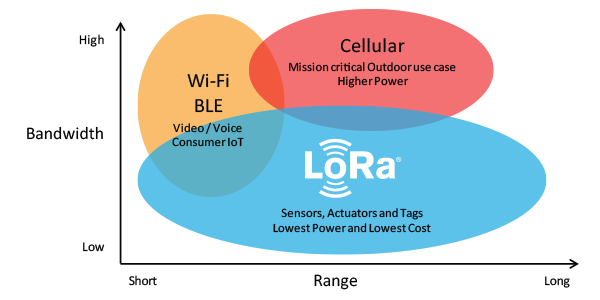
\includegraphics[width=1\textwidth]{figures/LoRa_context.png}
    \caption{LoRa vs other wireless technology\cite{lora_context}}
    \label{fig:lora_context}
\end{figure}

Figure~\ref{fig:lora_context} shows LoRa compared two other wireless technologies, Wi-Fi and cellular. Both Wi-Fi and cellular
are high in bandwidth with cellular having a longer range than Wi-Fi. They both have a much higher power consumption compared to LoRa.
LoRa has lower bandwidth but a high range. In a experiment during a TTN conference LoRa signals from a low orbit satellite were received~\cite{loa_satellite}.
On the other hand, as LoRa is designed for long range and low power, only few bytes are transmitted per day while Wi-Fi and cellular are capable of video streaming.
In urban areas LoRa has a range of 2-5 km and 15 km in suburban areas~\cite{limits_lora}.\\
LoRaWAN is not the same all around the world. There are regional parameters that come into play, one is for example the frequency band.
In Europe LoRaWAN operates on the in the 863-870MHz and 433MHz ISM band and in North America the 902-928MHz ISM band. Also channel bandwidth and maximum transmission 
settings are regulated by the government and thus are not the same for all regions~\cite{lora_wan_regional}.


\section{LoRaWAN architecture}
A LoRaWAN network architecture is a star-of-stars topology. The gateways relay the messages between the end-devices and a central network server.
Gateways are connected to the network server via IP connections, converting the RF packets to IP packets and vice versa~\cite{about_lora_wan}.
Network nodes are not associated with a specific gateway, rather messages sent by a node can be received by multiple gateways. Each gateway will then 
forward the the message to the network server who does the complex things such as filtering redundant packages, security checks, forwarding the messages
to the right application server etc.~\cite{what_is_lora_wan}.
As network communication is bidirectional, the network server is also responsible for scheduling responses to the end-nodes. There are different classes of 
end-nodes which will be described in the next section.

\begin{figure}[h]
    \centering
    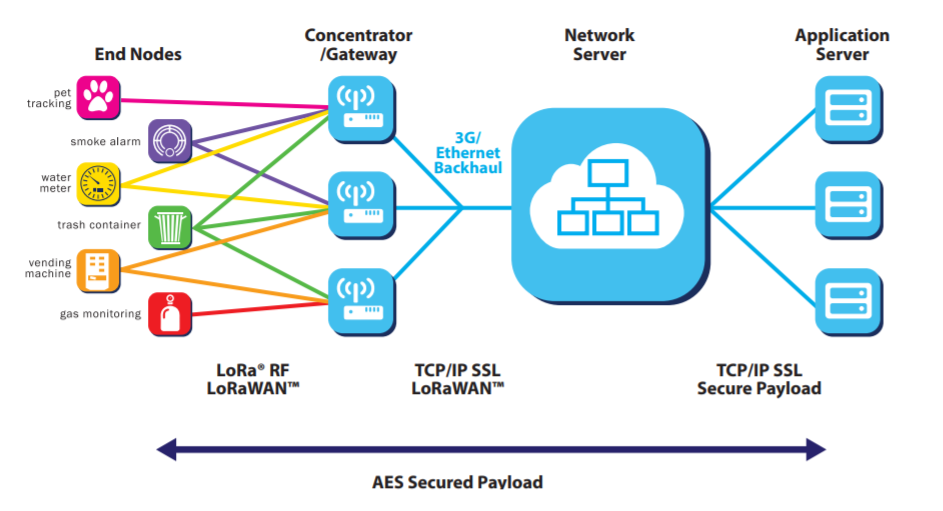
\includegraphics[width=1\textwidth]{figures/lorawan_network.png}
    \caption{LoRaWAN network architecture~\cite{what_is_lora_wan}}
    \label{fig:lorawan_network}
\end{figure}

As depicted in Figure~\ref{fig:lorawan_network}, the packets sent by end-devices (on the far left) such as alarms, tracking devices and monitoring devices,
can be received by multiple gateways. As the end-nodes are not linked to a particular gateway, the can be moved freely which is an important requirement for 
assets tracking.\\
The Figure also shows how security is built into LoRaWAN. The payload is end-to-end encrypted from the end-nodes to the applications server.
A unique 128-bit network session key is shared between  the end-device and the network server and 
another 128-bit application session key is shared end-to-end at the application level~\cite{about_lora_wan}.
With those measures LoRaWAN prevents eavesdropping. Spoofing is prevented by a MIC (Message Integrity Code)
in the MAC payload, and replay attacks are prevent by utilizing frame counters~\cite{lora_security}.


\section{End-node Classes}
There are three classes of end-devices. The following description is adapted from the LoRa Alliance guide~\cite{about_lora_wan,what_is_lora}:
\begin{itemize}
    \item Class A, Lowest power, bi-directional end-devices:\\
    \\
    This is the default class, supported by all LoRaWAN devices.
    It is always the end-node that initiates the communication. After an uplink
    two downlink windows open for the end-device to receive a response, enabling bi-directional communication.
    Either the first is used, or the second, but not both receive windows.
    The end-device can rest in low-power sleep mode, wake up when it needs to send a packet, receive a response
    in the downlink window, then go back to seep. This is an ALOHA-type of protocol. Class A devices have the lowest 
    power consumption. Downlinks from the server have to wait for an uplink from end-device and cannot be initiated directly.
    \item Class B, Bi-directional end-devices with deterministic downlink latency:\\
    \\ 
    Additionally to Class A receive windows, a Class B device opens extra receive windows at scheduled times.
    This is achieved by time-synchronized beacons from the gateway to the end-device to notify the end-device
    to open a receive window.

    \item Class C, Lowest latency, bi-directional end-devices:\\
    \\
    Devices of this class have always open receive windows, except for when they are themselves transmitting.
    A downlink transmission can be initiated by the network server at any time (assuming the device is not currently transmitting)
    resulting in no latency. Class C devices however use the most energy. They are more suitable for plugged in devices rather than
    battery powered devices.

\end{itemize}

\newpage


\section{LoRa signal (uplink)}
\subsection{Chirps}
A LoRa signal is a series of so called chirps as LoRa is derived from the Chirp Spread Spectrum modulation (CSS) technique. 
There are up-chirps and down-chirps. In CSS chirps are deliberately spread across the available bandwidth. Up-chirps go from low frequency 
to high frequency and down-chirps go from high frequency to low frequency. In Europe the LoRaWAN bandwidth for is 125 kHz. Assuming a center
frequency of 868.5 MHz, which is in the european ISM band, a full up-chirp, so called sweep, would go from 868.4375 MHz to 868.5625 MHz.

\begin{figure}[h]
    \centering
    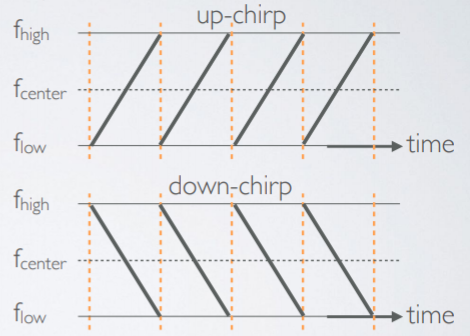
\includegraphics[width=0.6\textwidth]{figures/chirp_mobilefish.png}
    \caption{Up- and down chirps~\cite{lora_chirp_mobilefish}}
    \label{fig:chirp_mobilefish}
\end{figure}

Figure \ref{fig:chirp_mobilefish} shows the linear frequency increase resp. decrease over time over the full bandwidth
for up-chirps and down-chirps. Data is encoded by frequency jumps in the chirps. 

\begin{figure}[h]
    \centering
    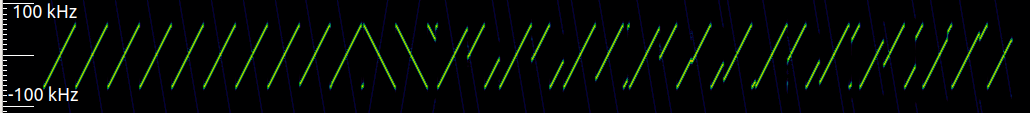
\includegraphics[width=1\textwidth]{figures/signal_Goodbye!_SF9_CR4_5.png}
    \caption{Own recording of uplink transmission by arduino equipped with a LoRa shield}
    \label{fig:Goodbye}
\end{figure}

The LoRa signal shown in~\ref{fig:Goodbye} carries the message  "Goodbye !". This message was sent 
with a spreading factor (SF) of 9 and coding rate of 4/5. The terms spreading factor and coding rate 
will be discussed later on.\\
As one can see, a typical LoRa signal start with a so called preamble, which are the 10 up-chirps at 
the beginning. Those are followed by two down-chirps, which signify the end of the preamble and the start 
of the actual payload. In this payload is a header, the actual encoded message followed by a Cyclic Redundancy Check (CRC).
The CRC is used for error correction.
\subsection{Symbol and Spreading Factor}
A LoRa signal holds various symbols. A symbol encodes one or more bits of data.
The spreading factor determines the number of encoded bits in a symbol.
In the shown recording one symbol holds 9 bits of data as the spreading factor of that signal was set to 9.
It follows that a symbol has $2^{SF}$ values. Those values range from 0 to 511 in case of SF 9. A sweep signal of SF 9
thus has 512 chips (no to be confused with chirps)~\cite{lora_symbol_mobilefish}.
The chips go linearly from low to high and then wrap around once the maximum frequency is reached.
\\
In Figure~\ref{fig:fict_symbols} a fictional symbol with SF 7 is shown. This particular 
arrangement of chips highlighted in orange would denote the symbol "1011111". Those 7 bits correspond 
to the decimal value 95.
\begin{figure}[h]
    \centering
    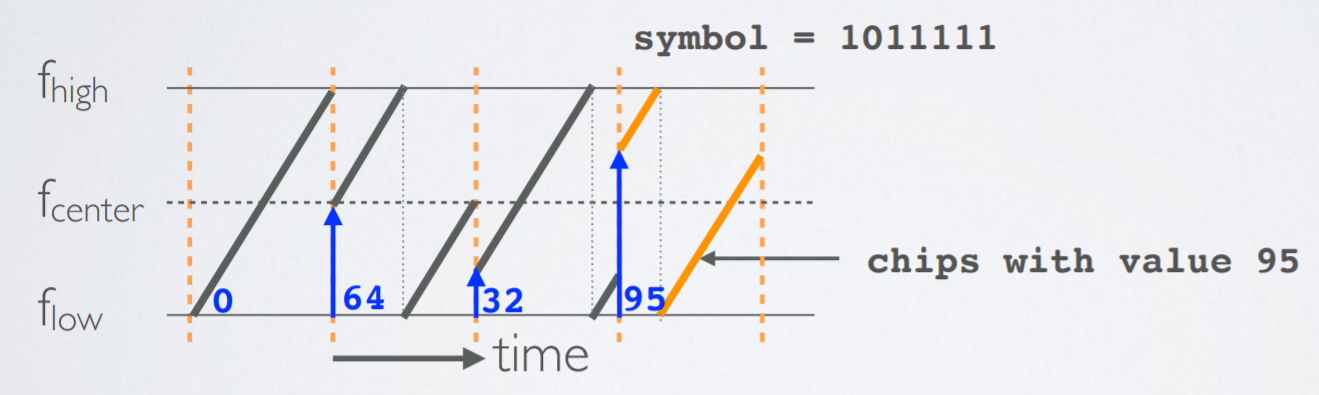
\includegraphics[width=1\textwidth]{figures/chips_and_symbols.png}
    \caption{Chips and symbols value~\cite{lora_symbol_mobilefish}}
    \label{fig:fict_symbols}
\end{figure}

In Figure \ref{fig:Goodbye_decoded}, a real world example is shown. The same LoRa signal as in Figure~\ref{fig:Goodbye} with SF 9 with the message "Goodbye !"
run through modified version of the LoRa decoder by Robyns et al.~\cite{robyns} and then through a python script where we match the samples to the symbols and their 
values. The last symbols encodes the hex value 142 which corresponds to these 9 bits "101000010". In a SF 9 signal each symbol encodes 9 bits.
\begin{figure}[h]
    \centering
    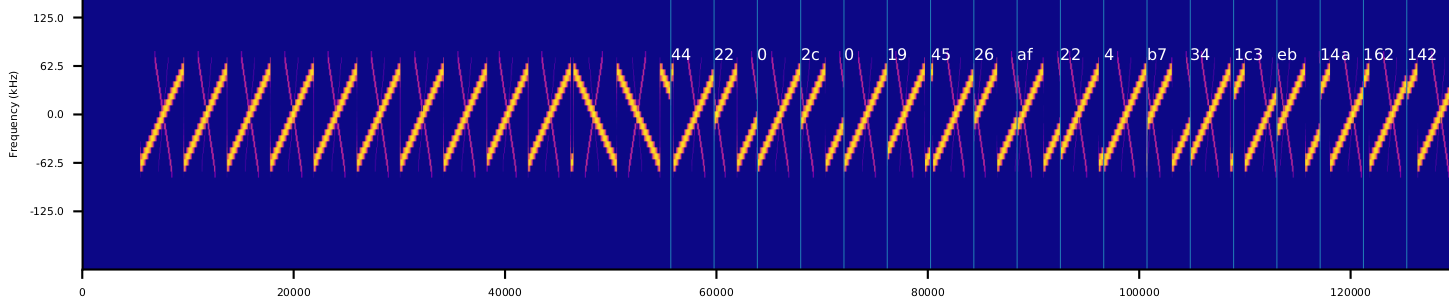
\includegraphics[width=1\textwidth]{figures/Goodbye_decoded.png}
    \caption{Running the signal through our toolchain, matching symbols with samples}
    \label{fig:Goodbye_decoded}
\end{figure}

\newpage

\subsection{Coding Rate}
LoRa signals are encoded with a coding rate (CR). The CR denotes the proportion of how many bits carry actual information. The bits that do not carry information are used 
for Forward Error Correction. The formula for coding rate is $CR=4/(4 + CR)$ where CR $\in \{1,2,3,4\}$. A CR of 1 is thus the proportion of 4/5 of actual information over 
bits used for error correction\cite{SX_design_guide,coding_rate_mobilefish}.
With FEC, corrupted bits e.g. due to interference can be corrected. With CR of 4, corresponds to $4/8 = 1/2$, half the transmitted bits carry information, the other half is for FEC.
The higher the CR (from 1-4) the more bits can get corrupted and corrected by FEC.
On the other hand, the higher the CR the more bits need to be transmitted which drains the battery more.


\subsection{Spreading Factor \& Time on Air}
The longer the packet, the longer the transmission time. LoRa packets can be shortened
by sending packets with implicit header mode where the
no header is sent and the settings that would have been specified in the header have to be 
predefined manually on the end device.\\
Assuming constant packet size and same bandwidth, varying the spreading factor increases resp. decreases the time on air.
The higher the SF, the longer the time on air. Higher SF means longer range. The spreading factor goes from 7 to 12. SF 7 has 
the shortest range, SF 12 the longest. The spreading factor essentially sets the duration of a chirp, a full sweep~\cite{exploratory_eng}.
\\
The symbol time is defined in the LoRa Design guide by $T_{sym} = \frac{2^{SF}}{BW}$~\cite{SX_design_guide}.
It follows as stated above, that the higher the SF the longer the symbol duration. Also, the higher the bandwidth (BW) the shorter
the symbol duration. In Europe the BW is 125~kHz, while in North America a BW of 500~kHz is allowed.
It also follows that with an increase in SF by 1 the symbol duration is doubled. The bit rate $R_{b}$  is then defined by 
$R_{b} = SF*\frac{[\frac{4}{4 * CR}]}{[\frac{2^{SF}}{BW}]}$ with CR being the coding rate for the error correction scheme~\cite{lora_modulation_basics}.
It follows from the formula that the higher the coding rate the lower the bit rate as with a higher CR more redundancy is added 
for the error correction scheme. Highest data rate for $BW=125~kHz$ and $CR=1$ is achieved 
with SF 7 resulting in a data rate of 5.5 kbits/s and the lowest data rate is achieved with SF 12 resulting in a data rate 0.29 kbits/s.
\\
The spreading factors are orthogonal to each other, meaning signals on different spreading factors do not interfere with each other. This is 
Code Division Multiple Access (CDMA) where a shared medium i.e. the bandwidth is optimized for multiple access.
\\
To optimize network capacity LoRaWAN employs a method called Adaptive Data Rate (ADR). With ADR the network server signals 
the end-device which spreading factor to use according to some measurements including the signal to noise ratio. Assuming there are multiple devices near a gateway 
that transmit with SF 12. This occupies the bandwidth for device that are farther away and actually need SF 12.
The network server detects that the nearby devices do not need a spreading factor of 12 and signal them to use 
a lower SF such as SF 7 or SF 8. The ADR setting has to be enabled on the end-devices and can be disabled.

\subsection{Packet structure}
The base form of a LoRa packet starts with the preamble, followed by the optional header with a header CRC, followed by the payload and finally the 
payload CRC. The number of payload symbols is calculated by the following formula~\cite{SX_design_guide}:\\ \\
$payloadSymbNb = 8 + max{(ceil(\frac{8PL-4SF+28+16-20H}{4(SF-2DE)})*(CR+4),0)}$ 
\\ \\

\begin{figure}[h]
    \centering
    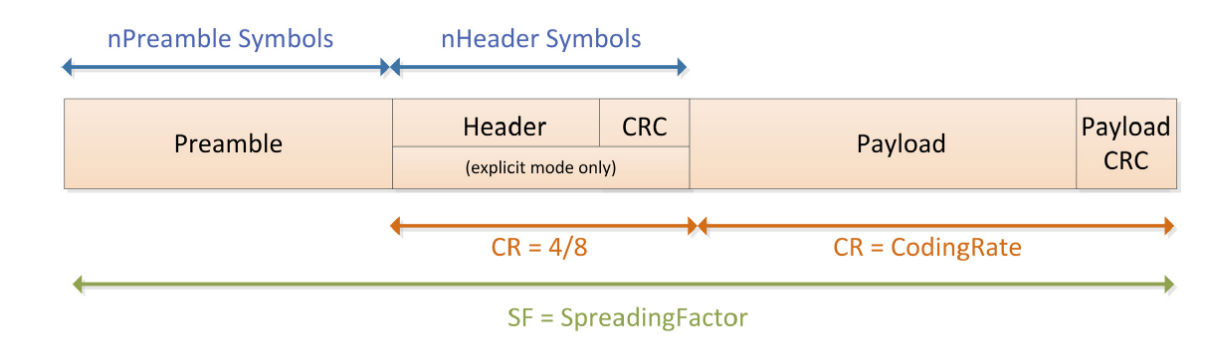
\includegraphics[width=1\textwidth]{figures/packet_struct.png}
    \caption{LoRa packet structure~\cite{SX_design_guide}}
    \label{fig:packet_struct}
\end{figure}

With: 
\begin{enumerate}
    \item PL being the number of payload bytes
    \item SF being the spreading factor
    \item H = 0 if header is enabled and H = 1 if no header
    \item DE = 0 if low data rate optimization is enabled and DE = 0 if disabled
    \item CR being the coding rate
    
\end{enumerate}

This website \url{https://www.loratools.nl/#/airtime} has an online tool for calculation the airtime.

As Figure~\ref{fig:packet_struct} shows, the header is always encoded with the highest coding rate, $CR=4$.
This is because the header contains crucial information such as the packet length.

Figure \ref{fig:uplink_struct} and Figure \ref{fig:downlink_struct} show the structure of an uplink resp. a 
downlink packet. There is no CRC in downlink packets. PHDR stands for PHY header.
Those are "raw" LoRa packets. LoRaWAN packets have additional fields such as MAC header (MHDR) and 
frame header (FHDR). Those are all in PHY payload of the "raw LoRa" packet as Figure~\ref{fig:lora_wan_struct} 
shows.   
\begin{figure}[h]
    \centering
    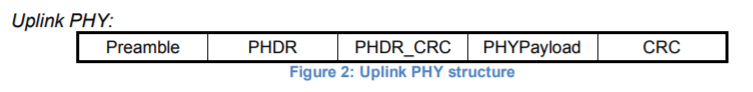
\includegraphics[width=1\textwidth]{figures/uplink_struct.png}
    \caption{LoRa uplink packet structure~\cite{lora_wan_spec}}
    \label{fig:uplink_struct}
\end{figure}

\begin{figure}[h]
    \centering
    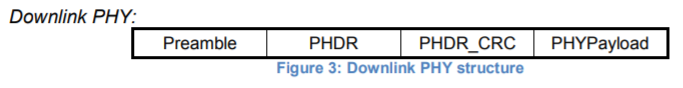
\includegraphics[width=1\textwidth]{figures/downlink_struct.png}
    \caption{LoRa downlink packet structure~\cite{lora_wan_spec}}
    \label{fig:downlink_struct}
\end{figure}

\begin{figure}[h]
    \centering
    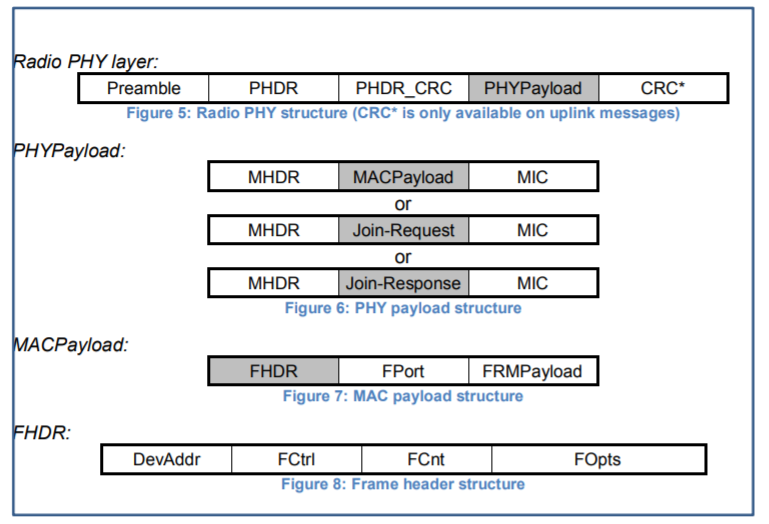
\includegraphics[width=1\textwidth]{figures/lorawan_struct.png}
    \caption{LoRaWAN packet~\cite{lora_wan_spec}}
    \label{fig:lora_wan_struct}
\end{figure}


\chapter{LoRa in SDRs}
Software-defined radios (SDR) implement components that are usually implemented in hardware.
The most popular signal processing frameworks is GNU Radio
For LoRa we were looking for an existing implementation that demodulates, and also modulates LoRa signals.

\section{Existing implementations}
There are three existing implmentations we looked at:
\begin{itemize}
    \item Josh Blum's LoRa Mod -and Demodulator for LoRa in the Pothos framework \url{https://myriadrf.org/news/lora-modem-limesdr/}
    \item Matt Knight's GNU Radio Module \url{https://github.com/BastilleResearch/gr-lora}
    \item Robyns et al. LoRa Module for GNU Radio \url{https://github.com/rpp0/gr-lora}
\end{itemize}

We tried Blum's implementation in the Pothos  first. The Pothos projects is an open source data-flow framework
supporting SoapySDR, a general framework for supporting SDR devices~\cite{pothos}.
Unfortunately the LoRa modem demo application did not work for at all. After spending a few unsuccessful days 
trying to get to the issue we moved to Knight's application.

Matt Knight held a great talk on reverse engineering LoRa at the GNU Radio conference 2016 \url{https://www.youtube.com/watch?v=-YNMRZC6v1s}.
GNU Radio, as Pothos, is a framework for signal processing.\\
From the GNU Radio website:
\begin{displayquote}
    GNU Radio is a free \& open-source software development toolkit that provides signal processing
    blocks to implement software radios. It can be used with readily-available low-cost external
    RF hardware to create software-defined radios, or without hardware in a simulation-like environment.
    It is widely used in research, industry, academia, government, and hobbyist environments to support both wireless
    communications research and real-world radio systems.~\cite{gnuradio}
\end{displayquote}

GNU Radio already comes with a wide set of blocks. Extensions are called Out Of Tree modules (OOT) as they are not in the 
standard tree of blocks. Knight's implementation did not work well for us. If we got an output from the decoder, it was not 
what was expected. A reason could be that in his examples the signal source block is an USRP SDR while we had a LimeSDR mini 
at our disposal. Simply switching the source blocks probably is not enough. We did not investigate the compatability between LimeSDR mini
and and USRP further but moved on to the final implementation.
His blocks are in modular fashion. The demodulator and decoder are separate blocks. Channelization and fine tuning must be done 
explicitly before passing the stream to the demodulator block.

\begin{figure}[h]
    \centering
    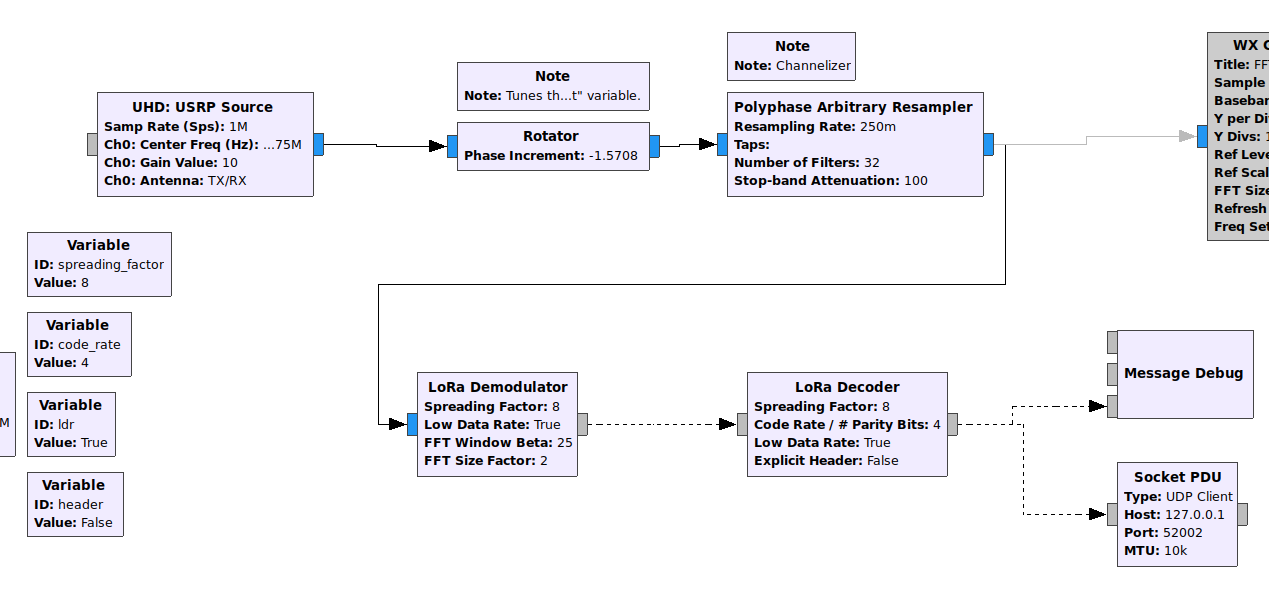
\includegraphics[width=1\textwidth]{figures/matt_gnu_example.png}
    \caption{Knight's GNU Radio gr-lora OOT RX example~\cite{knight_implementation}}
    \label{fig:knight_gnu}
\end{figure}

Figure~\ref{fig:knight_gnu} shows the typical flow of a GNU Radio flowgraph where data is passed 
from block to block as a stream (blue connection ports) or as message blocks (grey connection ports).
\\
Robyns' implementation is also an OOT module for GNU Radio. It has a elaborate 
installation and usage guide. A docker environment is also provided for testing the 
decoding of a LoRa signal, which is a big plus. Unlike Knight's implementation, this module
has demodulation, decoding and channelization all in one single block as shown in Figure~\ref{fig:robyns_gnu}. 
The module has been tested with various SDR devices but not with the LimeSDR mini. Nevertheless it worked
well for us and we based the CRAN implementation for LoRa on this module.


\begin{figure}[h]
    \centering
    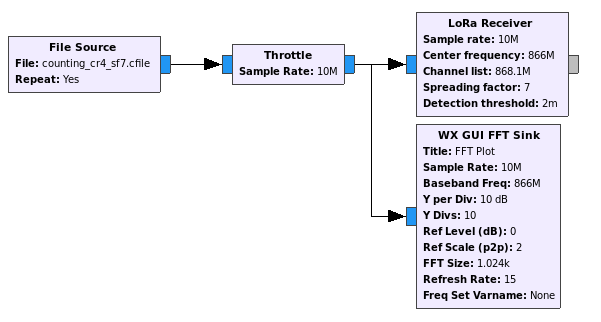
\includegraphics[width=0.8\textwidth]{figures/robyns_gnu.png}
    \caption{Single LoRa Receiver block (top right)~\cite{robyns_implementation}}
    \label{fig:robyns_gnu}
\end{figure}


\section{LoRa decoding}
The difficulty with reverse engineering LoRa is that its proprietary and
there is no official documentation on the PHY. To reverse engineer, information hints
on the PHY layer have to be taken from various official LoRaWAN documents, from patents, and the 
rest is guesswork. To make it more difficulty, some of the documentation is a lie as the PHY is not implement 
in the way it is described. 
complete lie, see Knight~\cite{knight_youtube}. 
The data is encoded before it is sent over the air to make it more resistant against interference.
Thus after demodulating the signal with a Fourier Transform, the data has to be decoded to make it usable.
Semtech's european patent hints at the following four steps:
\begin{enumerate}
    \item Symbol gray indexing. This adds error tolerance
    \item Data whitening. This induces randomness.
    \item Interleaving. This scrambles the bits within a frame
    \item Forward Error Correction. This adds correction parity bits.
    
\end{enumerate}
Those are 4 distinct operation which have to be reverse engineered~\cite{knight_youtube}.\\
Robyns et al. identified and implemented the following seven steps in their receiver to 
receive and decode a LoRa signal: detection, synchronization, demodulation, deinterleaving, dewhitening,
decoding, and packet construction~\cite{robyns_implementation}. They also provide a detailed description of the 
packet structure, especially the header. They deduce that because the minimum SF is SF 7, and the header is always 
transmitted mit CR = 4, it must fit in an interleaving matrix of a certain size which results int the header heaving a size of 
40 bits. The header contains important data as the payload length, thus it makes sense that the header is always sent with the highest
coding rate.
At the time of Knight's talk, he did not decode the header. Robyns implementation is quite complete except for CRC checks of the payload and header
as well as decoding multiple channels simultaneously. 


\chapter{}{C-RAN in LTE}
advantages
graphics
\chapter{C-RAN for LoRa}
\label{chap:cran_for_lora}

\section{Goal}
The goal is to set up a minimal working environment for a LoRa C-RAN.
The gateway's functionality should separated into an RRH and BBU component and the 
BBU component should be virtualized and run on general purpose hardware. 
A simple network server should process the uplink message and schedule a response if required. From this setup 
basic network requirements can be derived and measured as well as costs estimated.

\section{Hardware}
An Arduino Mega 2560 with the Dragion LoRa Shield v1.4 is the end device, see Figure~\ref{fig:ard}.
A LimeSDR mini, Figure~\ref{fig:sdr}, serves as the receiver for the RRH.
The Raspberry Pi, Figure~\ref{fig:rasp} with a LoRa hat was used for testing up -and downlink signals, but not for the experiment itself. 
Its hat is the iC880A LoRaWAN concentrator for the 868MHz frequency.

\begin{figure}[H]
    \centering
    \begin{subfigure}[b]{0.25\textwidth}
     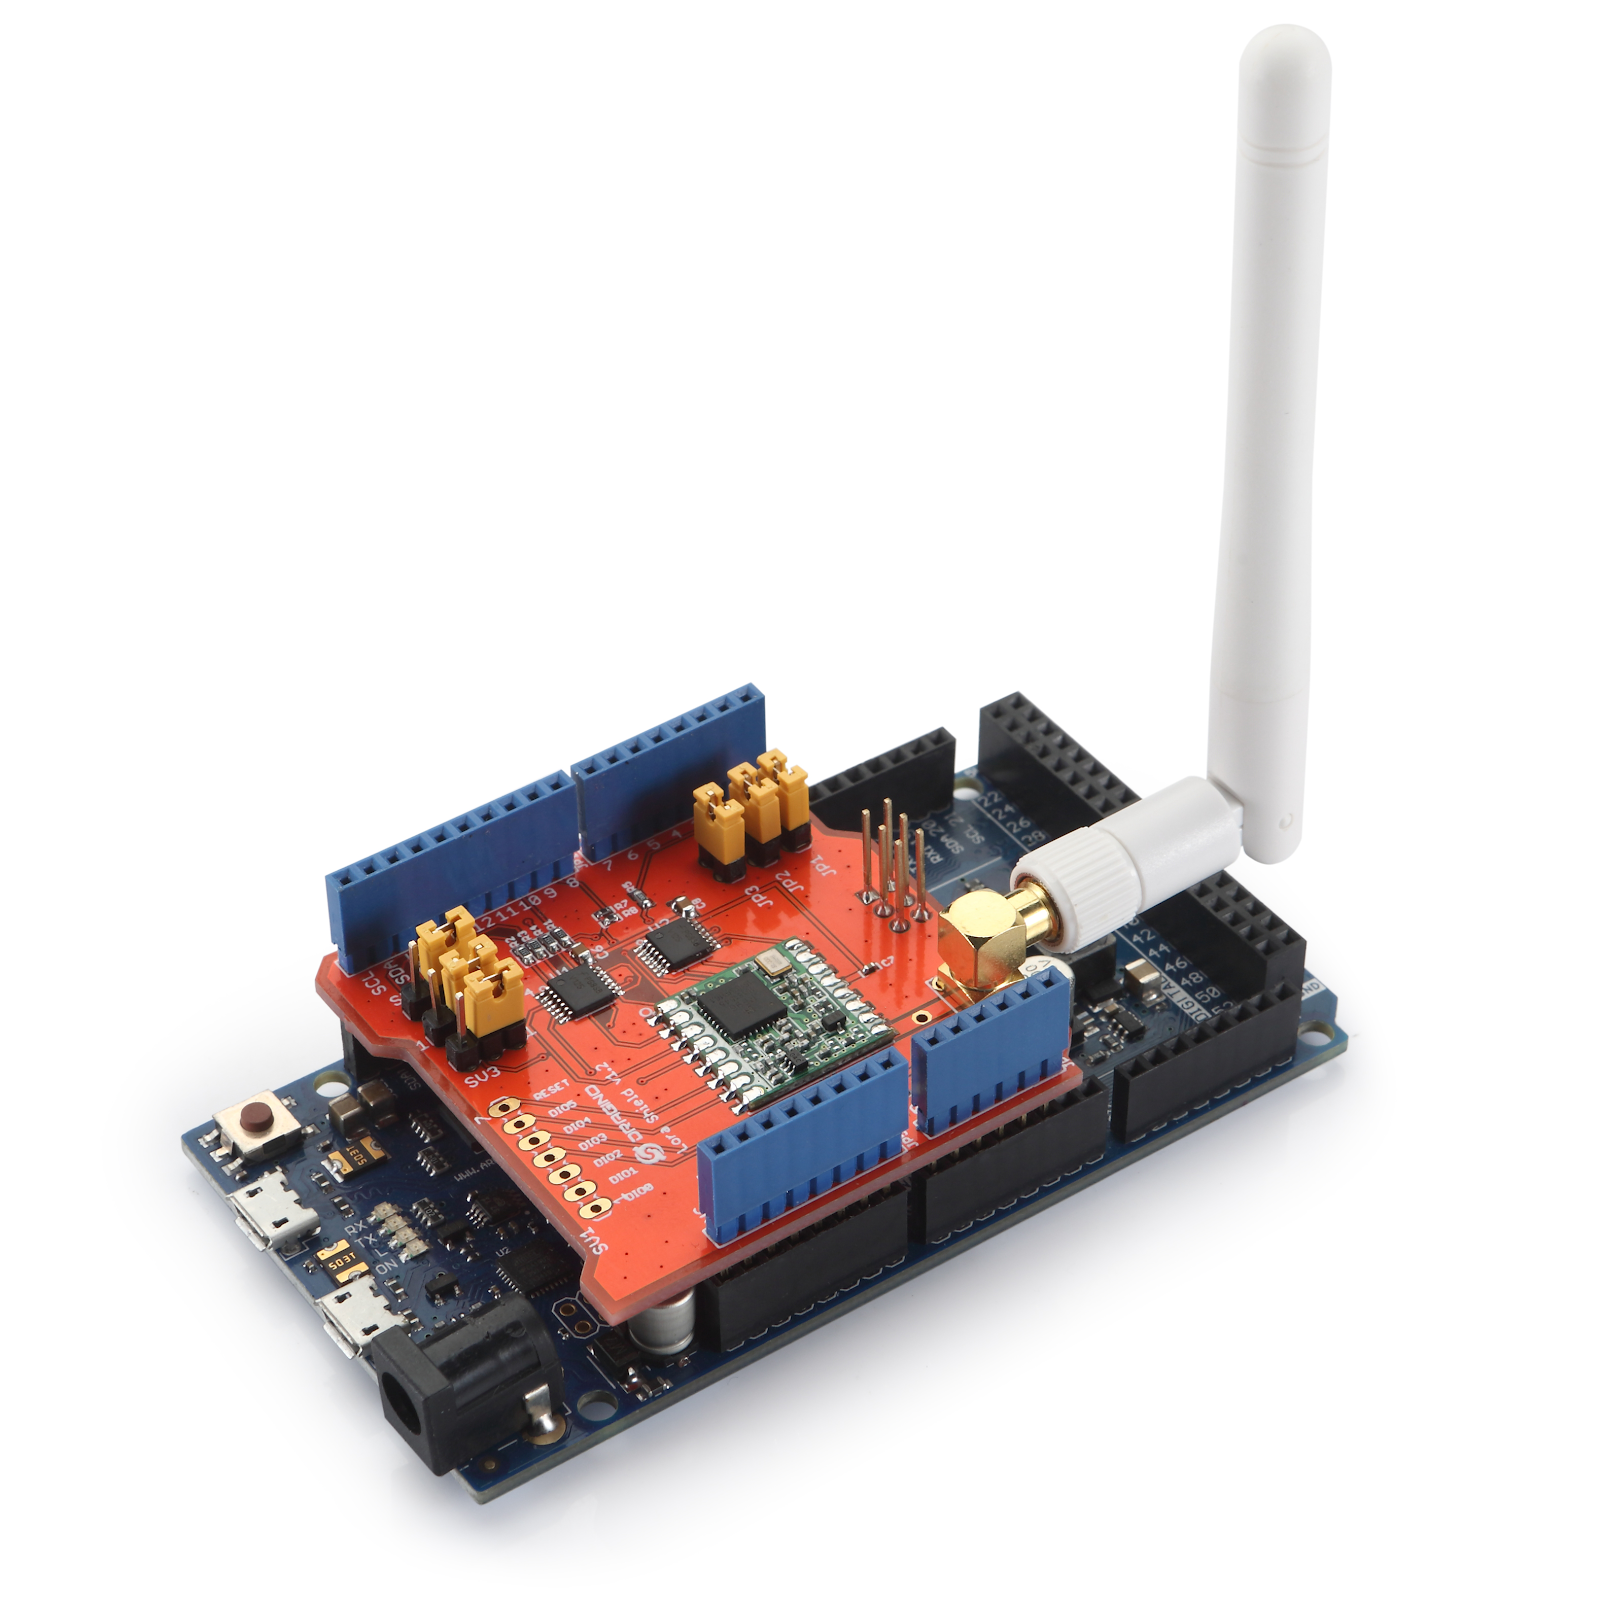
\includegraphics[width=1\textwidth]{figures/arduino.png}
     \caption{Arduino with LoRa shield}
     \label{fig:ard}
    \end{subfigure}%
    \hspace{2em}
    \begin{subfigure}[b]{0.25\textwidth}
     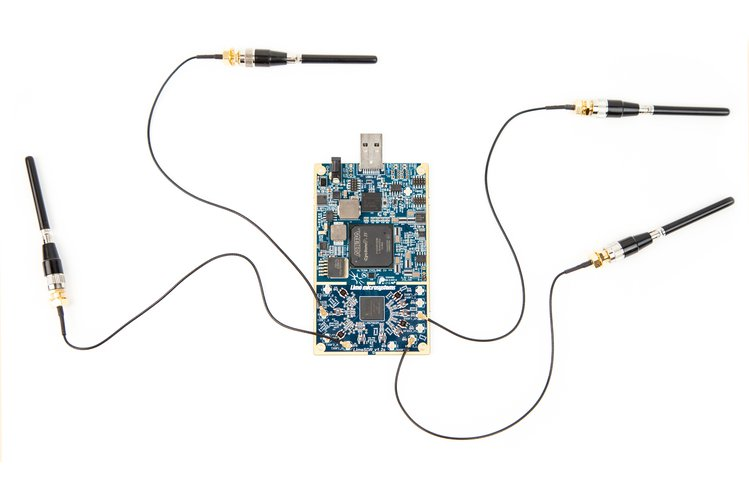
\includegraphics[width=1\textwidth]{figures/limesdr.png}
     \caption{LimeSDR mini}
     \label{fig:sdr}
    \end{subfigure}
    \hspace{2em}
    \begin{subfigure}[b]{0.25\textwidth}
     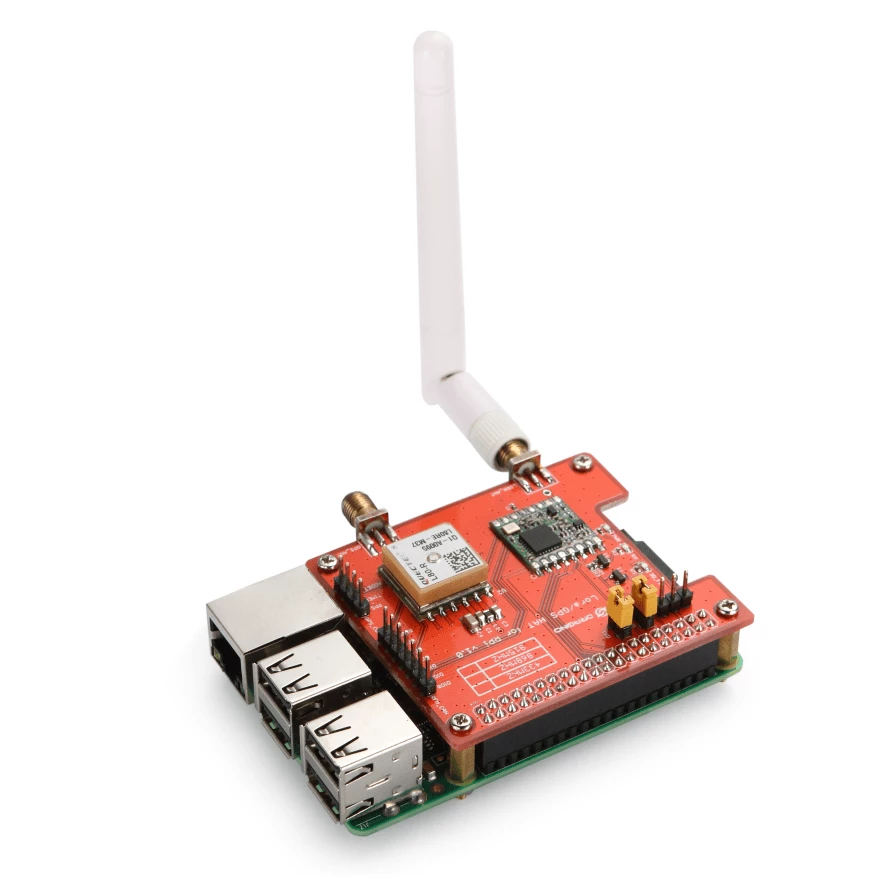
\includegraphics[width=1\textwidth]{figures/raspberry.png}
     \caption{Raspberry Pi with LoRa hat}
     \label{fig:rasp}
    \end{subfigure}
    \caption{Hardware devices}
\end{figure}
% getting a downlink signal
% recording from thethingsnetwrok
% recording from private networks
% manipualting private gateway
% offline generation of downlink signal see chapter

\section{Sending Uplink Signals}
Uplink signals are sent with an arduino device equipped with a LoRa shield. 
The arduino is controlled with an adapted form of the IBM LoraMAC-in-C (LMIC) library, modified to run on arduino devices.
Using this library we implemented a simple communication protocol where a queue of packets is sent out in an interval.
See section~\ref{sec:comm_prot} for detailed information.
% \url{https://github.com/matthijskooijman/arduino-lmic}.

\section{RRH and BBU}
For splitting up the LoRa gateway's functionality we use two laptops. 
One laptop has the LimeSDR mini plugged in and serves as the RRH. The other decodes the LoRa
signal in software, processes the signal and also generates LoRa signals in software and sends those downlink I/Q samples back to the RRH.
The processes on the second laptop run in virtualized environment with docker, more specifically docker compose, dockers orchestration tool.
\\
The LoRa OOT module by Robyns et al. has a branch called "encoder" where they began the implementation of modulating an uplink LoRa signal in software.
It is able to generate a specific test packet but the modulated signal has errors as we saw when we inspected the data payload on the LoRa gateway.
Having an uplink signal generator was a nice starting point, but we needed something to generate downlink signal. In the end we extended the existing implementation
by adding a downlink signal generation ability, see section~\ref{todo}.
\\
Though, as a first workaround we set up a private LoRaWAN network, scheduled a downlink, and recorded it to a file. Now we can stream that file as a response by streaming its content,
which are I/Q samples, to the RRH.


\section{Study Subjects}
\subsection{Network Utilization}
For measuring network traffic, the tool "bmon" is used which stands for bandwidth monitor.
It estimates the bits per second on all available network interfaces, ingoing as well as outgoing. 
\subsection{Impact of Delay}
Speed is essential for most communication systems.
LoRaWAN specifies two receive windows for class A devices. One 1 second after transmission, and if not
received in this window, another one 2 seconds after transmission.
The protocol for this experiment is more lenient. After transmission, the device starts listening
for at least 4 seconds before retransmitting the unacknowledged packet.
\subsection{Network Delay}
Using the command line tool \emph{netem}, which stands for network emulator, we introduce some delay between the RRH and the BBU.
The command is: tc qdisc add dev \emph{interface\_name} root netem delay 200ms. In which \emph{interface\_name} is something like 
eth0. 
\\
This instructs tc (traffic control) to modify the qdisc (queuing discipline) by 
adding (add) a new rule to the device (dev) e.g. eth0 to modify the outbound traffic scheduler (root) using 
the network emulator (netem) with a delay of 200ms~\cite{netem}.
\\
This setup can be easily seen an tested in action:
\begin{itemize}
    \item On the RRH add a delay of 8000ms
    \item On the BBU, in a terminal, type \emph{nc -l 4040}
    \item On the RRH, in a terminal, type \emph{nc <\emph{IP\_ADDRESS\_OF\_THE\_BBU}> 4040}
\end{itemize}

On the RRH on the same terminal on, type a message and send with enter. It should should arrive on the BBU's terminal 
after 8 seconds, which was the case. 

\subsection{Processing Delay}
Not only are network delays of importance, but also the processing time it takes for decoding incoming messages and scheduling downlink messages.
In the python script that sends the downlink, a call to \emph{time.sleep()} can simulate longer processing times.

\section{Architecture}
\subsection{Overview}
This section aims to first give a high level overview of the architecture and then give a more detailed 
architectural overview of each component.
Figure~\ref{fig:high_level_arch} shows the high level architecture with all the hardware components involved.
There are two laptops in the same network connected by an ethernet cable. One laptop serves as an RRH. It has the LimeSDR mini 
plugged into its USB port so it can send and receive signals.
\begin{figure}[h]
    \centering
    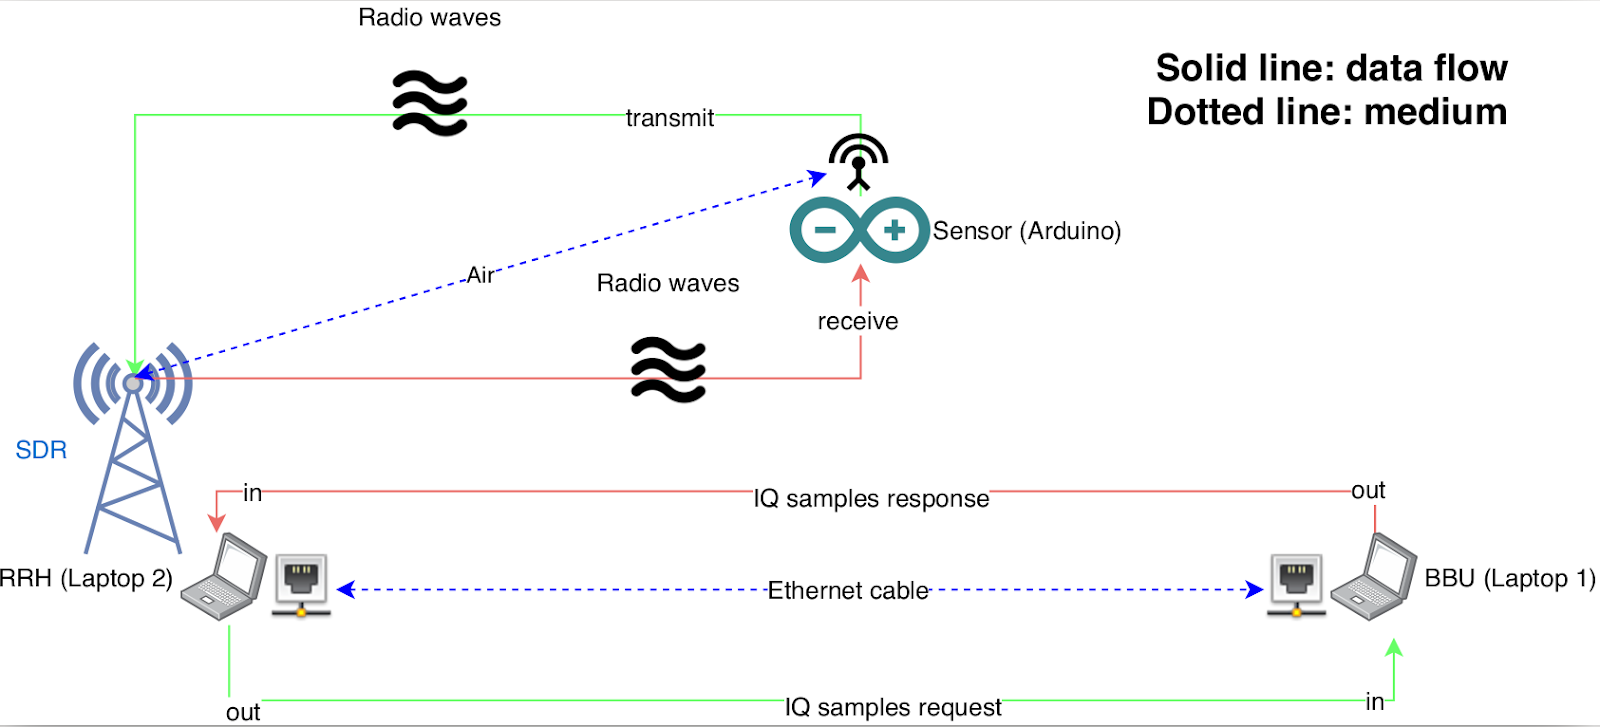
\includegraphics[width=1\textwidth]{figures/high_level_arch.png}
    \caption{High level architecture}
    \label{fig:high_level_arch}
\end{figure}
Incoming signals come from the arduino device. The arduino transmits packets over the air as radio waves. Those get picked up 
by the RRH which converts the analog signal and send them as digital 32bit floats as I/Q samples over ethernet to the second laptop.
This second laptop is the host for the virtual BBU that runs in a docker container. There the signals get demodulated and decoded.
Then the decoded signal gets processed. In case a response is requested, a response signal is generated and sent as I/Q samples back to the RRH.
From the it gets transmitted back to the arduino.
\subsection{Containerization and Orchestration}
docker docker compose, ready for cran as service openstack
\subsection{RRH and BBU}
The RRH is the simplest component. It has an antenna for input and one for output. In Figure~\ref{fig:seq_diagram} the RRH is composed by the two 
components "SDR RX" and "SDR TX". They correspond to the physical RX and TX slots ond the SDR device. The BBU is the "Lora Decoder" component. It runs 
in a virtualized environment. Decoded messages get passed to the "Python Script" component. This acts as a network server that schedules an acknowledgement
message back to the arduino. It could run on a third laptop connected via ethernet to the BBU laptop, but for our purposes it runs on the same laptop
as the BBU but in a separate docker container.
\begin{figure}[h]
    \centering
    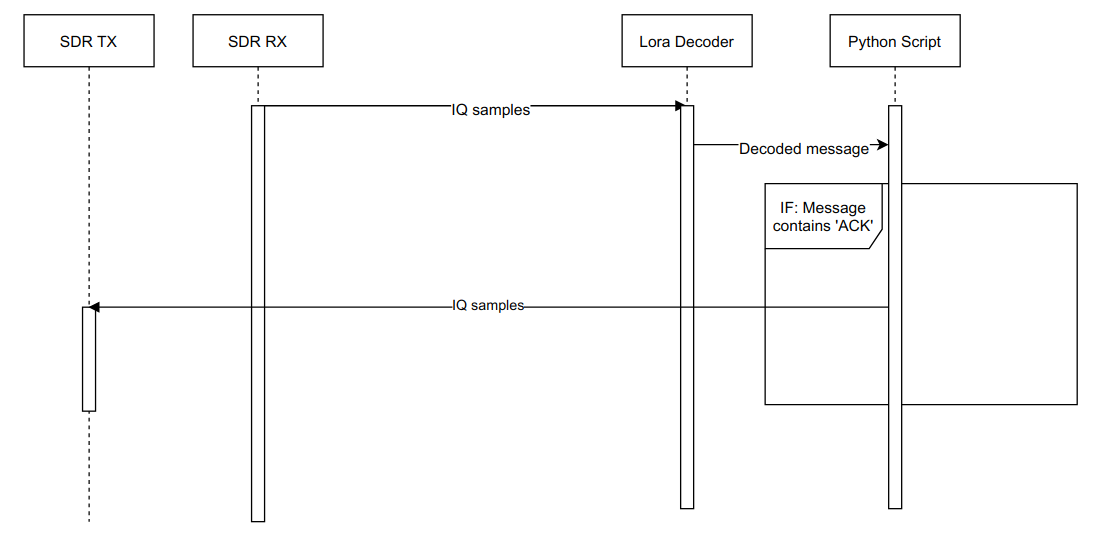
\includegraphics[width=1\textwidth]{figures/seq_diagram.png}
    \caption{Sequence diagram}
    \label{fig:seq_diagram}
\end{figure}


\section{Implementation}
All communication between the components happens over sockets. We use the ZeroMQ (ZMQ) networking library.
It is a good messaging library that offers N-to-N patterns as possible ways to connect the sockets, such as a request-reply pattern
or pub-sub pattern and many more~\cite{zeromq}.
GNU Radio offers ZMQ blocks out of the box, The TCP sink and source blocks for socket communication are still available but deprecated. 
For communication between the RRH and the BBU the pub-sub (publish-subscribe) pattern is used.
Figure~\ref{fig:seq_diagram} shows the "PUB" and "SUB" blocks and the data flow.
The RRH has a PUB sockets that takes as input the I/Q sample stream generated by the RX of the SDR.
The SUB socket in the BBU subscribes to this publishing socket. As this socket connection happens with TCP, the I/Q samples arrive in the order
they are sent an can be directly passed to the LoRa Decoder. Robyns' et al. implementation of LoRa Decoder sends the decoded message 
out on a UDP socket.  The "Python Script" block which is our LoRa network server takes the decoded messages over on this UDP socket and then, streams out 
I/Q samples of the response message over a ZMQ publishing socket to which the RRH's TX slot subscribes to. This closes the cycle.
One of the advantages of using ZMQ is that the sockets can be given the option to not time out or close. This means a subscribing socket 
can be started before a publishing socket without issues. The subscribing socket can wait for the publishing socket to get instantiated. For our architecture 
this means the docker containers for the RRH and BBU can be started in any order and more instances of the BBU can be added at runtime. The sub-pub pattern 
allows new subscribers and publisher to join.

\begin{figure}[h]
    \centering
    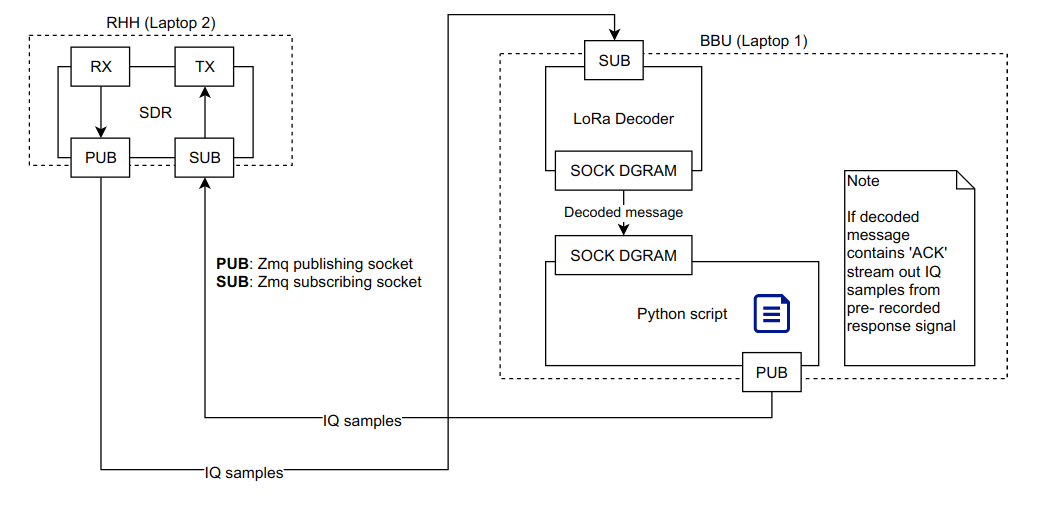
\includegraphics[width=1\textwidth]{figures/impl_diagram.png}
    \caption{Socket communication between components}
    \label{fig:impl_diagram}
\end{figure}

\subsection{RRH}
The RRH implementation is straightforward. Figure~\ref{fig:RRH_impl} show the necessary 
GNU Radio blocks. On the left is the RX block of the LimeSDR that streams the incoming signals to the 
PUB socket. The response message from the networks server to send out comes through a SUB socket which 
streams directly to the TX block of the LimeSDR on the far right of the Figure.
The parameter blocks allow the passing of command line arguments to the resulting application to configure
the socket addresses if necessary. As there is a OOT module needed for GNU Radio to work with the LimeSDR, a the 
RRH comes also in a docker container to quickly get started as the necessary dependencies have all been installed
in that container.
\begin{figure}[h]
    \centering
    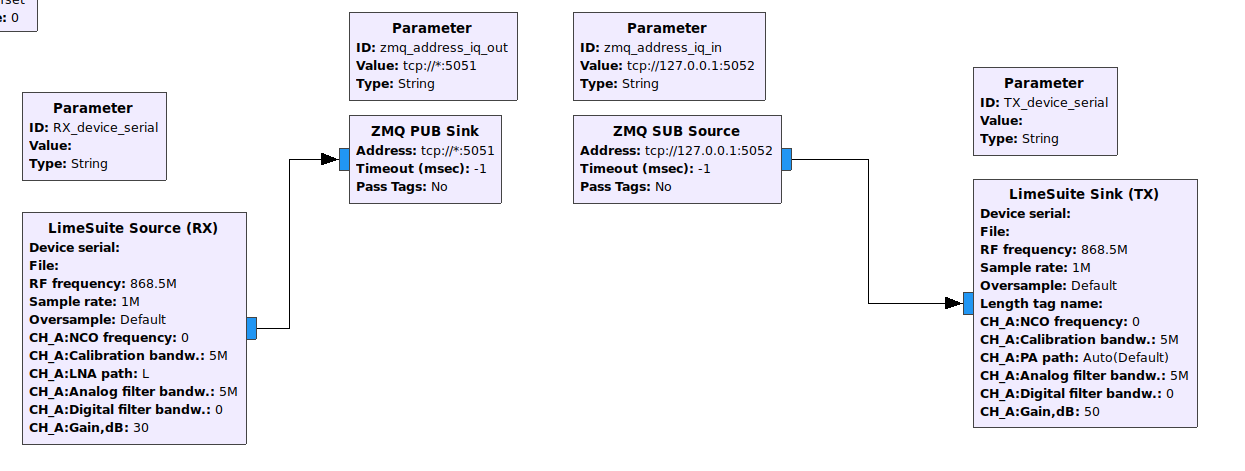
\includegraphics[width=1\textwidth]{figures/RRH_impl.png}
    \caption{GNU Radio blocks for the RRH}
    \label{fig:RRH_impl}
\end{figure}

\subsection{BBU}
The BBU as shown in Figure~\ref{fig:BBU_impl} takes in the RX stream of the RRH on a SUB socket,
passes the I/Q samples to the LoRa decoder. The decoder decodes LoRa signal and outputs them as a 
message on the message socket sink, far right in the Figure.


\begin{figure}[h]
    \centering
    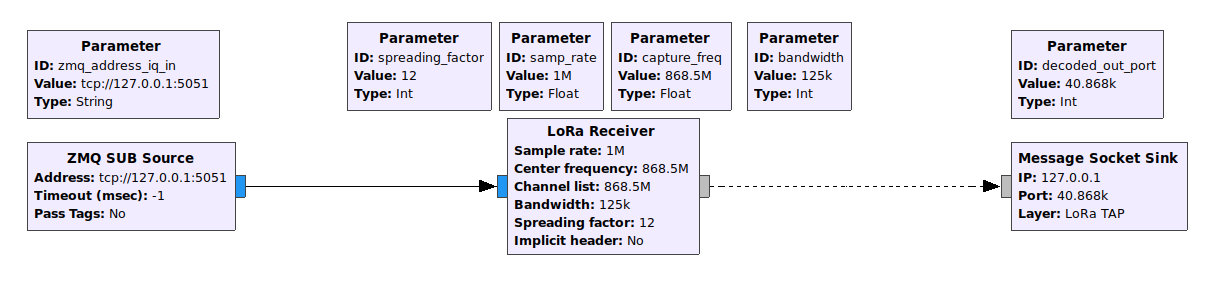
\includegraphics[width=1\textwidth]{figures/BBU_impl.png}
    \caption{GNU Radio blocks for the BBU}
    \label{fig:BBU_impl}
\end{figure}

The python script which acts as our network server, inspects the message payload and if an 
acknowledgement is required by the sender it generates the response signal. 
Listing~\ref{lst:python_code} shows an excerpt of that python script.
The acknowledgement message is a recording of a LoRa downlink signal. Its I/Q samples get read into memory.
The script connects to the UDP socket. As the BBU component and this python script run on the same host, it connects
to 127.0.0.1, the port is passed as argument to the script. As the focus lies on the split between RRH and BBU we decided
to hard code the IP address to localhost for the LoRa decoder and the network server as they run on the same machine as depicted 
in Figure~\ref{fig:impl_diagram}. 
Then, in an endless loop, data gets received from the socket. The buffer size is 1024 bytes.
Whenever "ACK" is in the message payload, the acknowledgement signal get streamed out over a ZMQ publishing socket.
\\
The BBU and the network server run each in a container started with docker compose.


\begin{listing}[h]
\begin{minted}[frame=single,linenos=false]{python}
import zmq
import socket
...
with open (dir_path + "/ACK_DOWN_SF12_CR4.raw") as f:
    ack = f.read()
...
zmq_socket = context.socket(zmq.PUB)
...
s = socket.socket(socket.AF_INET, socket.SOCK_DGRAM)
s.bind(("127.0.0.1", udp_port))
print ('listen for decoded lora packages on udp port ' + str(udp_port))
while True:
    data, addr = s.recvfrom(1024)

    if ("ACK" in data):
        zmq_socket.send(ack) 
    else:
        print ("received package requests no ACK")
     
    
    \end{minted}
    \caption{Excerpt of the python script that functions as the network server}
    \label{lst:python_code}
\end{listing}

\subsection{Communication Protocol Arduino}
\label{sec:comm_prot}

The LMIC library runs a loop that executes jobs scheduled to run at a specified time. 
In the \emph{setup()} function that runs once when the arduino starts settings such as 
the spreading factor, frequency and coding rate are set. The frequency is given in Hertz and the the datarate 
is set with a predefined enum from the LMIC library. Also, the initial job for the LMIC is initialized there, see 
Listing~\ref{lst::ard_setup} last line.

\begin{listing}[h]
    \begin{minted}[frame=single]{c++}
void setup() {
  Serial.begin(9600);
  ...
  // initialize runtime env
  os_init();
  ...
  
  LMIC.freq = 868500000;
  LMIC.txpow = 27; // Maximum TX power
  LMIC.datarate = DR_SF9;
  // This sets CR 4/5, BW125 (except for DR_SF7B, which uses BW250)
  LMIC.rps = updr2rps(LMIC.datarate);

  Serial.println("Started");
  Serial.flush();

  // setup initial job
  os_setCallback(&txjob, my_tx_func);
}
    \end{minted}
    \caption{Arduino setup() function}
    \label{lst::ard_setup}
    
\end{listing}

The last line schedules the initial job  \emph{txjob} with the \emph{my\_tx\_func} function that gets run
on execution of the job, see~Listing~\ref{lst::ard_mytx}. It takes the the index of the packet to send, Listing~\ref{lst::packets}, and
checks if the packet has "ACK" appended. Then the transmit function \emph{tx(packet, callback)} gets executed. 
It takes a packet and a callback function that gets executed after the transmission is finished. 
If an "ACK" is present, the callback function is set to \emph{my\_txdone\_func}, if not it is set to \emph{my\_txdone\_no\_ack\_func}.
Finally, in line 16 in Listing\ref{lst::ard_mytx}, schedules itself to be run again after \emph{TX\_INTERVAL} which is 4 seconds.


\begin{listing}[h]
    \begin{minted}[frame=single]{c++}
#define TX_INTERVAL 4000

int currentPacketIndex = 0;
const int numOfPackets = 3;
char *myPackets[numOfPackets] = {
    "This is packet 1ACK", 
    "This is packet 2ACK", 
    "This is packet 3",
};
    \end{minted}
    \caption{Packets 1 and 2 have "ACK" appended in their payload, while packet 3 does not}
    \label{lst::packets}
    
\end{listing}


\begin{listing}[h]
    \begin{minted}[frame=single, linenos]{c++}
static void my_tx_func(osjob_t *job) {
if (currentPacketIndex < numOfPackets) {
    ...
    char lastThree[3];
    memcpy(lastThree, &myPackets[currentPacketIndex][length - 3], 3);
    const char ack[] = {'A', 'C', 'K'};
    if (!memcmp(lastThree, ack, 3)) {
        // send and start rx for receiving ACK
        Serial.print("transmitting packet with ACK, packet: ");
        tx(myPackets[currentPacketIndex], my_txdone_func);
    } else {
        // send and schedule next packet
        Serial.print("transmitting packet without ACK, packet: ");
        tx(myPackets[currentPacketIndex], my_txdone_no_ack_func);
    }
    os_setTimedCallback(&txjob, os_getTime() +
                            ms2osticks(TX_INTERVAL), my_tx_func);
    } else {
        Serial.println("No more packets to send, done");
    }
}
    \end{minted}
    \caption{\emph{my\_tx\_fun} function}
    \label{lst::ard_mytx}
\end{listing}

The difference between the callback functions passed to the transmission function is that one
waits to receive an acknowledgement while the other simply increases the \emph{currentPacketIndex}
so the next packet gets sent the next time \emph{my\_tx\_func} get called.
The callback to the RX function gets executed every time a packets is received.
Listing~\ref{lst::ard_myrx} shows the implementation. The response signal by sent
by the network server has the payload "ACK", which is three bytes. 
If the \emph{LMIC.dataLen} is three bytes, it is assumed it is the expected acknowledgement signal.
The \emph{currentPacketIndex} gets incremented and the next transmission job gets set up.
Else, the \emph{currentPacketIndex} does not get incremented so the same packet gets rescheduled 
for transmission and the RX function gets called again.


\begin{listing}[h]
    \begin{minted}[frame=single, linenos]{c++}
static void my_rx_func(osjob_t *job)
{
    if (LMIC.dataLen == 3)
    {
    Serial.println("Got ACK");
    // if we get our ACK, start with next transmission, 
    // reschedules transmission at half TX_INTERVAL
    currentPacketIndex++;
    os_setTimedCallback(&txjob, os_getTime()
                            + ms2osticks(TX_INTERVAL / 2), my_tx_func);
    }
    else
    {
    Serial.println("NOT AN ACK");
    // resend packet if no ACK received within 3*TX_INTERVAL,
    // reschedules transmission in 3* TX_INTERVAL
    os_setTimedCallback(&txjob, os_getTime() 
                            + ms2osticks(3 * TX_INTERVAL), my_tx_func);
    // listen again
    rx(my_rx_func);
    }
}
    \end{minted}
    \caption{RX function that checks for the response or reschedules the packet transmission}
    \label{lst::ard_myrx}
\end{listing}

\section{Results}
\subsection{Network Utilization}
Monitoring the network utilization with bmon yields 
335 bytes per second on the ethernet network interface when idle. Once the C-RAN gets started the network
utilization rises to 8MiB/s (Mebibytes) which are equal to 67’108’864 bits.
Bmon only gives an estimation. The theoretical value can be derived the following way:
\\
\begin{itemize}
    \item The LimeSDR had the sample rate set to 1 million samples per second by default.
    \item The type is of complex type of 32 bit, (I/Q) => 2 x 32 bit, which gives 64 million~bits/s
    \item MTU (Maximum Transmission Unit) on most systems is 1500 bytes.
    \item Overhead for TCP and IP is 20 bytes each => 40 bytes
    \item This gives a MSS (Maximum Segment Size) of 1460 bytes
    \item 64M bits ÷ (1460 bytes×8) = 5479.45 packets needed
    \item Total overhead: 5480 packets x (40 bytes x 8) = 175360 bits
    \item 64’000’000 bits + 1’753’600 bits = 65’753’600 bit/s = 7.8 MiB/s
\end{itemize}

The RRH is constantly sending samples to the BBU. It does not matter if the arduino 
sends 1 signal every 4 seconds or 40 signals per second, the network utilization stays the same
as the sample rate stays the same. The experiment worked without error with the 
10 gigabit ethernet connection, but it did not work over Wi-Fi connection.
The response signal sent from the BBU to the RRH did not arrive on the RRH.
\\
\\
\textbf{Optimization}: The load on the network can be reduced. According to the Nyquist-Shannon sampling theorem~\cite{Shannon1949}
a sufficient sampling rate $f_{s}$ for a signal with bandwidth $B$ is given by:
\begin{center}
    $f_{s} > 2*B$  
\end{center}

The signal bandwidth of the LoRa signal sent with the Arduino is set to 125 kHz. Thus the minimum sampling frequency according to the formula above
is 250'000 samples per second which is a quarter of the previous sample rate of 1 million. This also quarters the network utilization from 8 MiB to 2 MiB, see Table~\ref{tabl:samprates}.
Lowering the sampling rate below the Nyquist-Shannon limit results in the signal not getting successfully decoded.
With the sample rate of 125'000 the maximum allowed signal bandwidth to reconstruct that signal is 62.5 kHz so the Arduino signal with 125 kHz bandwidth 
cannot get decoded, see last line in the Table.

\begin{table}[h]
    \centering
    \setlength{\tabcolsep}{22pt}
    \renewcommand{\arraystretch}{1.2}
    \begin{tabular}{cccc}
        \toprule
        Samples & Max. Signal & Network & Decode Success \\
        per second & Bandwidth & Utilization & in Experiment\\
        \midrule
        1'000'000  &500 kHz & 8 MiB/s    &yes\\
        500'000  &250 kHz & 4 MiB/s    &yes\\
        250'000&  125 kHz&  2 MiB/s  & yes\\
        125'000 & 62.5 kHz & 1 MiB/s & no\\
        \bottomrule
       \end{tabular}
\caption{Sampling rates and network utilization}
\label{tabl:samprates}
\end{table}

LoRaWAN defines different regional parameters. In the EU SF 8 to SF 12 signals are sent with 125 kHz bandwidth, while SF 7
can be sent with 125 kHz or 250 kHz bandwidth. In the US on the other hand SF 7 to SF 12 can also be sent with
a 500 kHz bandwidth \cite{lora_wan_reg_params}.
This has to be taken into consideration when designing a LoRaWAN compliant C-RAN architecture.
The network load for decoding a 500 kHz bandwidth US signal is for times higher than a EU 125 kHz bandwidth signal.

\subsection{Cost}
LoRa gateways come in various prices. The low cost indoor commercial gateway by TTN costs around 70\$ while their higher end 
gateway sells for 300\$. Cheaper gateways can be built with and Arduino and a LoRa shield such as the Dragino shield (22\$).
The issue is that those are often based on the SX1272/SX1276 chips. While cheaper, those gateways are so called single channel 
gateways. They can only listen on one channel with one spreading factor. They are not LoRaWAN compliant~\cite{single_chan_gate}.
LoRaWAN compliant gateways can be built with a Raspberry Pi with a iC880A concentrator (130\$) which use the SX1301/SX1257 chips. They can receive packets
of sent with different spreading factors on up to 8 channels in parallel.
\\
The LoRa Decoder block of Robyns et al. does not yet support multichannel decoding. Spreading factor and center frequency
need to be set explicitly, making it a single channel gateway. The advantage of having a decoder in software is that new instances 
of the LoRa Decoder block can be added without additional hardware costs. As the BBU is containerized, starting up a new instance 
is as easy as instructing docker to start a new instance of the decoder and pass it the desired frequency and SF. This saves the costs of 
a LoRaWAN concentrator.
These savings are offset by the need for general purpose hardware the containers can run on and the higher bandwidth requirements.

Using the amazon aws cost calculator \url{https://calculator.s3.amazonaws.com/index.html} the following three fields are of importance : 
\begin{itemize}
    \item Compute:
    \begin{itemize}
        \item  Amazon EC2 Instance
    \end{itemize}
    \item  Data Transfer:
    \begin{itemize}
        \item Data Transfer In
        \item Data Transfer Out  
    \end{itemize}
\end{itemize}

For the EC2 instance we select the \emph{a1.medium} which comes with 1 vCPU and 2 GiB of memory at \emph{0.0255\$} per hour.
\\
\\
Data Transfer In has to be 8 MiB/s to accommodate the maximum possible signal bandwidth of 500 kHz in the US or 
4 MiB/s for the maximal signal bandwidth of 250 kHz in EU. In this cost estimation example we proceed with 4 MiB/s for Europe.
4 MiB per second are 363 GB per day. Data input is free on AWS  giving a daily cost of 0\$.
\\
\\
Data Transfer Out on the other hand does cost. The amount of data that gets sent out depends on
how many uplink signals require a downlink signal. In our example a fixed 3 byte payload response is sent.
In LoRaWAN, downlink messages can have variable length, multiple bytes long.
Sticking with our example, the fixed downlink response signal with a payload of 3 bytes (excluding preamble, header and crc ), SF 7 and coding rate 4/5,
yields an I/Q sample stream of 248 kB (including preamble, header and crc) after modulation.
How many downlink signals will the required? That depends on wether the end-node requires a confirmed uplink.
However, there is an upper limit. The EU specifies a 1\% duty cycle for the 868.0 - 868.6 MHz frequency plan~\cite{duty_cycle}.
The downlink signal has an airtime of 25.86 ms. With a duty cycle of 1\% a downlink signal can be sent every 3 seconds.
This means a maximum of 28'800 downlink signals of this type can be sent by one gateway a day.
Data Transfer Out is thus limited to 7 GB a day if duty cycles are respected, $28800 * 248~kB = 7 GB$.
TTN encourages end-devices to not use confirmed uplinks as most gateways are not designed to send an receive
simultaneously. We assume for our experiment that about 30\% of total possible downlink signals need to be sent
which gives a Data Transfer Out of 2.1 GB/day.
\\
\\
Total monthly cost amounts to 24.07\$:
\begin{itemize}
    \item Compute:
    \begin{itemize}
        \item  Amazon EC2 Instance: 18.67\$
    \end{itemize}
    \item  Data Transfer:
    \begin{itemize}
        \item Data Transfer In: 0\$
        \item Data Transfer Out: 5.40\$  
    \end{itemize}
\end{itemize}

As the modulated signals have to ben sent out over TCP/IP from the BBU to the RRH, a TCP/IP overhead 
of 2.7\% could theoretically be added, but it is negligible as it is an estimation for 
comparison and not for absolute numbers.
\\
\\
In the traditional LoRa setup where the gateway is not split into and RRH and BBU 
component the decoded packet get sent to the network server and not the I/Q samples.
Assuming the same setup as before, instead of calculating $28800 * 248~kB = 7 GB$, the following
has to be calculated: 

\begin{itemize}
    \item payload size: 3 bytes
    \item header size: 4 bytes
    \item CRC size: 0 bytes, downlink messaged do not have a CRC
\end{itemize}

This yield the following $28800 * 7~Bytes = 0.0002016 GB$, which is an insignificant daily amount for AWS as
it gives already 0\$ as cost estimation before we even apply the 30\% usage assumptions.
Thus, sending the I/Q samples over the internet to the cloud is infinitely more expensive compared to just 
sending the demodulated signal. 
\\
However, in a local cloud setup where RRH and BBU are on the same network
or in a network architecture the data does not have to be routed over the internet and 
the BBU can still be virtualized and centralized in a BBU hotel for much cheaper.
In such a setup hardware and operational costs can be saved as outlined in section~\ref{sec:moving_to_cran}.
For each gateway at least 130\$ costs for the LoRa concentrator could be saved by doing its job in software.
For a hobbyist that operates a single gateway it may not be useful as now he needs to invest in general purpose hardware 
that is fast enough to do the decoding in software. Though, for an operator with multiple gateways, centralizing and virtualizing
the decoding has similar benefits as a C-RAN for LTE.

\subsection{Delays}
Various network delays for the outgoing sample stream from the RRH to the BBU were set.
Table~\ref{tabl:delay} summarizes the results.
\\
The higher the delay the less network utilization was measured with bmon. But only after delay,
namely 300ms. Without delay, RX resp. TX on the ethernet ports of the RRH and BBU is 8 MiB/s.
With a 800ms delay it is about 2.32 MiB/s. With a 400 ms delay it is 5.5 MiB/s. With a delay 
of 300ms or less bmon measured still 8 MiB/s.
\\
The expectation was that the signals would get decoded on the BBU the same as without delay just later.
However this was not the case. There was a difference between only a single signal being picked up by the RRH and sent 
to the BBU and the arduino sending multiple signals in an interval and the RRH sending I/Q samples of multiple signals 
to the BBU.
\\
For a delay of 500 ms and below the following held true in the experiment:
\\
\begin{itemize}
    \item The arduino sends a single signal then stops. The RRH receives the signal and sends the I/Q sample stream
    to the BBU. On the BBU the signal gets successfully decoded with a delay of 2 to 10 times the delay set with Netem.
    \item The arduino sends signals in a 4 second interval. The signals get decoded in order on the BBU.
\end{itemize}


For a delay of 500 ms and up the following held true in the experiment:
\\
\begin{itemize}
    \item The arduino sends a single signal then stops. The RRH receives the signal and sends the I/Q sample stream 
    to the BBU. On the BBU the signal does not get decoded.
    \item The arduino send signals in a 4 second interval. Some signals get decoded after the delay times 10. Some signals do not get decoded.
    In an experiment with 800 ms delay,  the first three signals did not get decoded, the fourth signal did after a 10 seconds delay. \\
    Generally, the first signals never got decoded, only the 4th or later signals got eventually decoded by the BBU.
    A possible cause could be that either the LorRa decoder block or the GNU Radio scheduler have an issue 
    with some sort of buffer not being filled fast enough when a single signal is sent and if multiple signals are sent 
    the buffer has time to fill up which leads to some decode success when multiple signals are sent in an interval.
    This is but pure speculation and would need to be investigated further.

\end{itemize}


\begin{table}[h]
    \centering
    \setlength{\tabcolsep}{22pt}
    \renewcommand{\arraystretch}{1.2}
    \begin{tabular}{SScc}
        \toprule 
            {\multirow{1}{*}[-2pt]{Netem Delay}} & {\multirow{1}{*}[-2pt]{Network Traffic }} & \multicolumn{2}{c}{Eventual Decode Success}\\ \cmidrule{3-4}
        
            {(ms)}&{(MiB/s)}&Single Signal & Signal Interval \\
            \midrule
            0  & 8  & yes & yes \\
            20  & 8 & yes & yes \\
            50  & 8 & yes & yes \\
            100  & 8 & yes & yes \\
            200  & 8 & yes & yes \\
            300  & 8 & yes & yes \\
            400  & 5.5 & yes & yes \\
            500  & 4.25 & no & yes \\
            600  & 3.6 & no & yes \\
            800  & 2.3 & no & yes \\
            1000  & 1.92 & no & yes \\
            \bottomrule
    \end{tabular}
    \caption{Effect of delay on network traffic on decode process}
    \label{tabl:delay}
\end{table}

\subsection{Processing Delay}
Processing delays on the LoRa network server were straightforward and as expected. 
Sleep is called in the Python script that sends the downlink. If this is more than the 
time the Arduino is set to listen for downlink signals, the downlink is missed.
For LoRaWAN class A devices this is 1 resp. 2 seconds after uplink.\\
In this example the Arduino sends in an interval of 4 seconds which is more than enough time under good conditions.
However if network delay and processign delays occurs, this changes.
With a Netem delay of 400 ms, the decoded message arrives about 3 seconds later, which leaves only 1 second for the downlink to be sent.


\chapter{LoRa Tools}


%\input{.tex}
%\input{.tex}
\chapter{Future work}
The design for a C-RAN for LoRa depends on level of sophistication of
software processing for LoRa. \\
Best case scenario would haven been if software decoding, encoding and the LoRaWan protocol
were already implemented for software defined radios.
\\
As this was not the case, we first had to spend a significant amount of time 
to understand the inner workings of LoRa better. This is made more difficult by the fact 
that the PHY layer of LoRa is proprietary and no official documentation exists.

\section{Limitations}
A first limitation is that the response signal is a recording of a real downlink signal and not 
purely generated in software on demand. Nevertheless we developed the tools to make it possible.
\\
Second, the LoRa protocol implemented on the Arduino is "raw" LoRa and not compliant 
with the LoRaWan standard. This was necessary as decoding a LoRaWan packet is not yet implement in 
the decoder, in terms of destructuring the received packet according to all the LoRaWan fields as shown
in Figure~\ref{fig:lora_wan_struct}.
\\
Third, the experiment, C-RAN architecture and Arduino implementation is based on the assumption 
of a single end-device and gateway in the network. In a LoRaWan, end-devices ignore downlink packets
not destined for them. Our Arduino however happily accepts any "ACK" downlink because of the premise that 
all downlinks are destined for it as it is the only device in the network.\\
Further in a network with multiple gateways, an uplink signal gets picked up by multiple gateways and 
forwarded to the network server. Then the network server discards duplicates and decides over which gateway
the downlink response is sent. In our network however there is only one RRH.

\section{Improvements}
Improvements to the protocol implementation can be made. Though, instead
of improving this protocol, it makes far more sense to adopt the LoRaWan protocol.
The LoRaWan protocol is an open protocol. Implementing it on the decoder requires the 
necessary time and knowledge. The Arduino could already speak the LoRaWan protocol with 
the help of the LMIC library which offers a fairly complete LoRaWan Class A device implementation.
\\
On network server side, an initial improvement would be to dynamically generate the response signal
by incorporating the encoder for downlink signals in the architecture.
\\ \\
Further, there is only one decoder / BBU running because there is only one Arduino sending on one channel.
As the BBU is containerized, the experiment can be run with multiple Arduino devices on different 
channels and spreading factor. Witch Docker compose, multiple BBUs could be started to handle the different 
channels and spreading factor, they would then forward the decoded messages to the network server.
This can be already done with the current implementation. The network server however could be replaced 
with the open implementation of the chirpstack network server, \url{https://www.chirpstack.io/network-server/overview/}. 
It handles among other things the de-duplication of LoRaWan messages and downlink scheduling.
It takes LoRaWan messages from an MQTT broker. MQTT like ZMQ facilitates architectures based on a publish-subscribe strategy. So instead of the decoder sending the decoded messages 
out over an UDP socket and our Python script subscribing, the decoder can publish the decoded message to the 
MQTT broker. For downlink scheduling the chirpstack network server sends the message also over MQTT
back to the gateway for modulation and transmission. For the C-RAN architecture where the downlink is modulated 
in software and not on the gateway anymore, this would need a redesign where the RRH simply receives the I/Q samples
to transmit without having to do any LoRa modulation. Then the chirpstack application server could be 
added for free, giving a nice web-interface similar to the TTN interface, but instead of 
traditional LoRaWan network architecture a C-RAN LoRaWan architecture is running.
\\ \\
For further developing the centralized / cloud aspect of C-RAN, the BBUs instead of running on a single host
controlled by Docker compose could be spread of multiple machines with Docker swarm or Kubernetes. 
Further down the road BBU and network server could be offered as a service via software such as Openstack 
essentially providing C-RAN as a service as demonstrated for LTE by in~\cite{Nikaein2015}.
\\ \\
Finally, it needs to be investigated why the decoder cannot successfully decode I/Q samples of a single signal streamed over and ethernet connection as TCP/IP packets 
if a network delay of more than 500ms is emulated on the connection. Also, there are some open issues on the 
GitHub repo of the decoder and a few items that are not yet implemented such as multichannel decoding and 
CRC checks for payload and header. However, the decoder itself is not in scope of this thesis and is just mentioned here for 
completeness.



\chapter{Summary and Conclusions}



% \begin{thebibliography}{99}
% \addcontentsline{toc}{chapter}{Bibliography}

% \bibitem{label} Autoren: Titel, Verlag, \url{http://...}, Datum.

% \end{thebibliography}

\nocite{*}
\bibliographystyle{ieeetr}
\bibliography{references}




\chapter*{Abbreviations}
\addcontentsline{toc}{chapter}{Abbreviations}
\markboth{ABBREVIATONS}{}


\abr{C-RAN}{Centralized / Cloud Radio Access Network}
\abr{CAPEX}{Capital Expenditures}
\abr{CSS}{Chirp Spread Spectrum}
\abr{IP}{Internet Protocol}
\abr{LAN}{Local Area Network}
\abr{LoRa}{Long Range}
\abr{LTE}{Long-Term Evolution}
\abr{OPEX}{Operational Expenditures}
\abr{PHY}{Physical}
\abr{RF}{Radio Frequency}
\abr{RX}{Reception}
\abr{SDR}{Software Defined Radio}
\abr{TCP}{Transport Control Protocol}
\abr{TTN}{The Things Network}
\abr{TX}{Transmission}
\abr{WAN}{Wide Area Network}


\chapter*{Glossary}
\addcontentsline{toc}{chapter}{Glossary}
\markboth{GLOSSARY}{}


\begin{description}
  \item[Authentication] 
  \item[Authorization] Authorization is the decision whether an entity is allowed to perform a particular action or not, 
       e.g. whether a user is allowed to attach to a network or not.
  \item[Accounting]
\end{description}


\addcontentsline{toc}{chapter}{List of Figures}
\listoffigures
\addcontentsline{toc}{chapter}{List of Tables}
\listoftables

\appendix

\chapter{Installation Guidelines}
For Docker, see~\ref{run-with-docker}.
For manual installation, see~\ref{manual-installation-ubuntu}

\chapter{Contents of the CD}
The CD contains the following:

\begin{itemize}
    \item a folder with the arduino source code
    \item a folder for the docker setup
    \item a folder with the grc (gnuradio companion) files
    \item a folder with various signal recordings
    \item a folder with the thesis source code and the final thesis pdf
    \item a folder with various tools for decoding, encoding and visualization of LoRa signals
    \item a README.md file
\end{itemize}

\emph{All contents of the CD are available online on my GitHuB \url{https://github.com/mustard123/master-thesis}}


\chapter{README.md}
Below is the README.md file converted to \LaTeX. It is
recommended to view the file in a markdown viewer e.g. VS Code or on GitHub \url{https://github.com/mustard123/master-thesis}

\section{C-RAN for LoRa}\label{c-ran-for-lora}

An Arduino with a LoRa shield sends out packets over the air in an
interval. Some packets require an acknowledgment (ACK). If an ACK is
required, the Arduino waits for a certain amount of time for the ACK. If
the ACK arrives in time, the Arduino starts transmitting the next
packet. If not, the Arduino will resend the packet and again wait for
the ACK.

The RRH (Remote Radio Head) receives radio waves with a LimeSDR. The RRH
streams the IQ samples over the network the the BBU (Base Band Unit).

The BBU decodes the message. If the message says it require and ACK, the
BBU send out IQ samples of the ACK message over the network to the RRH
which transmits them back over the air to the Arduino.

\subsection{Run with Docker}\label{run-with-docker}

\begin{enumerate}
\def\labelenumi{\arabic{enumi}.}
\tightlist
\item
  Clone the repo
\item
  Go to the docker directory
\end{enumerate}

\subsubsection{\texorpdfstring{\textbf{\emph{Info}}}{Info}}\label{info}

\begin{itemize}
\tightlist
\item
  The container run in priviledged mode to easily access plugged in USB
  devices
\item
  The container run in network mode host (No NAT or Bridge has to be
  considered). This means the containers have the ip address of the host
  machine. If RRH and BBU run on different machines, find out their
  respective IP with \emph{ifconfig} and pass the address as arguments
  in the docker-compose.yml, see below.
\end{itemize}

\begin{center}\rule{0.5\linewidth}{\linethickness}\end{center}

\subsection{RRH}\label{rrh}

In the RRH directory run:

\begin{verbatim}
docker-compose up 
\end{verbatim}

This starts the Remote Radio Head. The RRH looks for a LimeSDR, it
prints errors if it cannot find one. You can plug one in after the
container has started and it should get detectet. By default it uses the
first LimeSDR it can find.

\subsubsection{Parameters}\label{parameters}

There are various parameters which you can specify in the
\emph{docker-compose.yml} file.

Run this to see what the possible params are:

\begin{verbatim}
./zero_mq_split_a.py -h
\end{verbatim}

Output:

\begin{verbatim}
Usage: zero_mq_split_a.py: [options]

Options:
  -h, --help            show this help message and exit
  --RX-device-serial=RX_DEVICE_SERIAL
                        Set RX_device_serial [default=]
  --TX-device-serial=TX_DEVICE_SERIAL
                        Set TX_device_serial [default=]
  --capture-freq=CAPTURE_FREQ
                        Set capture_freq [default=868.5M]
  --samp-rate=SAMP_RATE
                        Set samp_rate [default=1.0M]
  --zmq-address-iq-in=ZMQ_ADDRESS_IQ_IN
                        Set zmq_address_iq_in [default=tcp://127.0.0.1:5052]
  --zmq-address-iq-out=ZMQ_ADDRESS_IQ_OUT
                        Set zmq_address_iq_out [default=tcp://*:5051]
\end{verbatim}

\begin{longtable}[]{@{}ll@{}}
\toprule
\begin{minipage}[b]{0.18\columnwidth}\raggedright\strut
Param\strut
\end{minipage} & \begin{minipage}[b]{0.18\columnwidth}\raggedright\strut
Explanation\strut
\end{minipage}\tabularnewline
\midrule
\endhead
\begin{minipage}[t]{0.18\columnwidth}\raggedright\strut
RX-device-serial\strut
\end{minipage} & \begin{minipage}[t]{0.18\columnwidth}\raggedright\strut
By default, the program will use the first LimeSDR it can find for
receiving and transmitting signal. If you have two devices you can
specify which should receive by passing the device Serial (See section
\textbf{Help} for more info)\strut
\end{minipage}\tabularnewline
\begin{minipage}[t]{0.18\columnwidth}\raggedright\strut
TX-device-serial\strut
\end{minipage} & \begin{minipage}[t]{0.18\columnwidth}\raggedright\strut
By default, the program will use the first LimeSDR it can find for
receiving and transmitting signal. If you have two devices you can
specify which should transmit by passing the device Serial (See section
\textbf{Help} for more info)\strut
\end{minipage}\tabularnewline
\begin{minipage}[t]{0.18\columnwidth}\raggedright\strut
capture-freq\strut
\end{minipage} & \begin{minipage}[t]{0.18\columnwidth}\raggedright\strut
The frequency in Hz at which the RRH listens for signals. Default value
is 86850000\strut
\end{minipage}\tabularnewline
\begin{minipage}[t]{0.18\columnwidth}\raggedright\strut
samp-rate\strut
\end{minipage} & \begin{minipage}[t]{0.18\columnwidth}\raggedright\strut
How many samples per second. Default value is 1000000. Must be at least
double the bandwidth of the expected signal see \emph{Nyquist-Shannon
principle}\strut
\end{minipage}\tabularnewline
\begin{minipage}[t]{0.18\columnwidth}\raggedright\strut
zmq-address-iq-in\strut
\end{minipage} & \begin{minipage}[t]{0.18\columnwidth}\raggedright\strut
ZMQ address to which the RRH subscribes to receive an IQ samples stream
(from the BBU) to then send out (TX). Default value is
tcp://127.0.0.1:5052 meaning the IQ samples are expected to come from
localhost on port 5052. Normally RRH and BBU are on different devices
but on the same network\strut
\end{minipage}\tabularnewline
\begin{minipage}[t]{0.18\columnwidth}\raggedright\strut
--zmq-address-iq-out\strut
\end{minipage} & \begin{minipage}[t]{0.18\columnwidth}\raggedright\strut
ZMQ address on which the RRH streams out the IQ samples (to the BBU) it
receives (RX). Default is tcp://*:5051 meaning it publishes the stream
on all interface on port 5051\strut
\end{minipage}\tabularnewline
\bottomrule
\end{longtable}

\begin{center}\rule{0.5\linewidth}{\linethickness}\end{center}

To pass the parameters you have to specify them in the
docker-compose.yml

Example:

To pass a capture frequencey of 915M and a sample rate of 250k enter the
params in the following way in the command field:

\emph{docker-compose.yml}

\begin{verbatim}
version: '3'
services:
    rrh:
        build: .
        privileged: true
        network_mode: host
        volumes:
                - /dev/bus/usb:/dev/bus/usb
        command: ["--capture-freq", "915000000", "--samp_rate", "250000"]
\end{verbatim}

\begin{center}\rule{0.5\linewidth}{\linethickness}\end{center}

\subsection{BBU}\label{bbu}

The BBU has two components: * LoRa\_Decoder: receives a stream of IQ
samples from the RRH, decodes the LoRa signal and sends the decoded
message out on a UDP socket * LoRa\_Network\_Server: receives the
messages from that UDP socket and, depending on message content, streams
response IQ samples to the RRH or does not give a response

In the BBU directory run:

\begin{verbatim}
docker-compose up 
\end{verbatim}

This starts both components of the BBU

\subsubsection{Params}\label{params}

The LoRa\_Decoder has the following params:

\begin{verbatim}
Usage: zero_mq_split_b.py: [options]

Options:
  -h, --help            show this help message and exit
  --bandwidth=BANDWIDTH
                        Set bandwidth [default=125000]
  --capture-freq=CAPTURE_FREQ
                        Set capture_freq [default=868.5M]
  --decoded-out-port=DECODED_OUT_PORT
                        Set decoded_out_port [default=40868]
  --samp-rate=SAMP_RATE
                        Set samp_rate [default=1.0M]
  --spreading-factor=SPREADING_FACTOR
                        Set spreading_factor [default=12]
  --zmq-address-iq-in=ZMQ_ADDRESS_IQ_IN
                        Set zmq_address_iq_in [default=tcp://127.0.0.1:5051]
\end{verbatim}

\begin{longtable}[]{@{}ll@{}}
\toprule
\begin{minipage}[b]{0.18\columnwidth}\raggedright\strut
Param\strut
\end{minipage} & \begin{minipage}[b]{0.18\columnwidth}\raggedright\strut
Explanation\strut
\end{minipage}\tabularnewline
\midrule
\endhead
\begin{minipage}[t]{0.18\columnwidth}\raggedright\strut
bandwith\strut
\end{minipage} & \begin{minipage}[t]{0.18\columnwidth}\raggedright\strut
The bandwidth in Hz of the LoRa signal. Default is 125000.\strut
\end{minipage}\tabularnewline
\begin{minipage}[t]{0.18\columnwidth}\raggedright\strut
capture-freq\strut
\end{minipage} & \begin{minipage}[t]{0.18\columnwidth}\raggedright\strut
The frequency in Hz of the LoRa signal. The RRH of course must also
listen on this frequeny. Default is 868500000.\strut
\end{minipage}\tabularnewline
\begin{minipage}[t]{0.18\columnwidth}\raggedright\strut
decoded-out-port\strut
\end{minipage} & \begin{minipage}[t]{0.18\columnwidth}\raggedright\strut
On which port the decoded messages will be sent out. Localhost only. The
LoRa\_Network\_Server needs to be configured to listen on this port.
Default is 40868.\strut
\end{minipage}\tabularnewline
\begin{minipage}[t]{0.18\columnwidth}\raggedright\strut
samp-rate\strut
\end{minipage} & \begin{minipage}[t]{0.18\columnwidth}\raggedright\strut
How many samples per second to expect from the RRH. Default is
1000000\strut
\end{minipage}\tabularnewline
\begin{minipage}[t]{0.18\columnwidth}\raggedright\strut
spreading-factor\strut
\end{minipage} & \begin{minipage}[t]{0.18\columnwidth}\raggedright\strut
The spreading factor of the incoming LoRa signal. From {[}7-12{]}
inclusive. Default is 12\strut
\end{minipage}\tabularnewline
\begin{minipage}[t]{0.18\columnwidth}\raggedright\strut
--zmq-address-iq-in\strut
\end{minipage} & \begin{minipage}[t]{0.18\columnwidth}\raggedright\strut
ZMQ address to which the BBU subscribes to receive an IQ samples stream
(from the RRH) to decode. Default value is tcp://127.0.0.1:5051 meaning
the IQ samples are expected to come from localhost on port 5051.
Normally RRH and BBU are on different devices but on the same
network\strut
\end{minipage}\tabularnewline
\bottomrule
\end{longtable}

\begin{center}\rule{0.5\linewidth}{\linethickness}\end{center}

The LoRa\_Network\_Server has the following params:

\begin{verbatim}
usage: lora_socket_server.py [-h] [-o OUT_PORT] [-i INPUT_PORT]

Connect to udp port for receiving decoded LoRa signals, if an ACK is required
publish ACK iq samples via zmq socket for Remote Radio Head to receive and
send out (TX).

optional arguments:
  -h, --help            show this help message and exit
  -o OUT_PORT, --out-port OUT_PORT
                        zmq port to publish downstream (i.e ACK) iq samples
                        (default: 5052)
  -i INPUT_PORT, --input-port INPUT_PORT
                        UDP port to connect for receiving decoded lora
                        messages (default: 40868)

\end{verbatim}

\begin{longtable}[]{@{}ll@{}}
\toprule
\begin{minipage}[b]{0.18\columnwidth}\raggedright\strut
Param\strut
\end{minipage} & \begin{minipage}[b]{0.18\columnwidth}\raggedright\strut
Explanation\strut
\end{minipage}\tabularnewline
\midrule
\endhead
\begin{minipage}[t]{0.18\columnwidth}\raggedright\strut
out-port\strut
\end{minipage} & \begin{minipage}[t]{0.18\columnwidth}\raggedright\strut
Publish the response IQ samples on all interface on this port. Default
is 5052. (The response is 3 bytes long (``ACK'') and SF 12. This is
hardcoded for now)\strut
\end{minipage}\tabularnewline
\begin{minipage}[t]{0.18\columnwidth}\raggedright\strut
input-port\strut
\end{minipage} & \begin{minipage}[t]{0.18\columnwidth}\raggedright\strut
UDP port to receive the decoded messages sent by the LoRa\_Decoder.
Default is 40868\strut
\end{minipage}\tabularnewline
\bottomrule
\end{longtable}

\begin{center}\rule{0.5\linewidth}{\linethickness}\end{center}

To pass the parameters you have to specify them in the
docker-compose.yml file.

Example:

To have the LoRa\_Decoder send the decoded messages out on port 30300
and the Lora\_Network\_Server to listen on port 30300 accordingly pass
the arguments like below to the respective command field:

\emph{docker-compose.yml}

\begin{verbatim}
version: '3'
services:
        lora_decoder:
                build: ./LoRa_Decoder
                network_mode: host
                tty: true
                command: ["--decoded-out-port", "30300"]
        lora_network_server:
                build: ./LoRa_Network_Server
                network_mode: host
                tty: true
                command: ["--input-port", "30300"] 
\end{verbatim}

\subsection{LimeSDR}\label{limesdr}

\begin{itemize}
\tightlist
\item
  Plug in the antennas on the LimeSDR board on \emph{RX1\_L} and
  \emph{TX1\_1}
\end{itemize}

\subsection{Help}\label{help}

\begin{itemize}
\item
  LimeSDR calibration/gain error:
\item
  \href{https://wiki.myriadrf.org/Lime_Suite}{Download LimeSuite
  Toolkit} to calibrate the LimeSDR
\item
  LimeSDR find device serial:
\item
  With LimeSuite installed run \emph{LimeUtil --find}
\item
  Or run \emph{lsusb -v} and look for the LimeSDR device
\end{itemize}

\begin{center}\rule{0.5\linewidth}{\linethickness}\end{center}

\section{Arduino}\label{arduino}

\textbf{The arduino-lmic library is required
\href{https://github.com/matthijskooijman/arduino-lmic}{Instructions
here}}

\begin{enumerate}
\def\labelenumi{\arabic{enumi}.}
\tightlist
\item
  Go to the arduino directory.
\item
  Compile and upload the code to the arduino
\item
  The arduino runs the protocol in the manner described at the
  beginning.
\item
  It send packets with SF9 and expects the ACK response to be SF12 as
  well.
\item
  After 3 packets the arduino has finished.
\item
  Look at the Serial output for details. Baud rate 9600
\end{enumerate}

\textbf{Info}

PlatformIO was used to compile and upload the image to the arduino.

\begin{center}\rule{0.5\linewidth}{\linethickness}\end{center}

\subsection{Manual installation
Ubuntu}\label{manual-installation-ubuntu}

Visit this guide for
\href{https://wiki.myriadrf.org/Gr-limesdr_Plugin_for_GNURadio}{installing
LimeSDR Plugin for GNU Radio} for more detail. This guide only has the
short version.

Install dependencies for signal processing:

\begin{verbatim}
sudo apt-get update && sudo apt-get install -y gnuradio=3.7.11-10 libboost-all-dev swig git cmake software-properties-common \
libcppunit-1.14-0 libfftw3-bin libvolk1-bin liblog4cpp5v5 python libliquid1d libliquid-dev python-pip \
&& pip install numpy && pip install scipy
\end{verbatim}

Install LimeSuite

\begin{verbatim}
sudo add-apt-repository -y ppa:myriadrf/drivers && sudo apt-get update \
&& sudo apt-get install -y limesuite liblimesuite-dev limesuite-udev limesuite-images \
soapysdr-tools soapysdr-module-lms7
\end{verbatim}

Clone and install LimeSDR Plugin for GNU Radio:

\begin{verbatim}
git clone https://github.com/myriadrf/gr-limesdr && cd gr-limesdr && mkdir build && cd build && cmake .. && make && sudo make install && sudo ldconfig
\end{verbatim}

Clone and install rpp0's LoRa decoder for gnuradio

\begin{verbatim}
git clone https://github.com/rpp0/gr-lora.git && cd gr-lora && git checkout b1d38fab9032a52eaf31bf33a145df45fce7512f\
&& mkdir build && cd build \
&& cmake .. && make && sudo make install \
&& cd .. && rm -rf build \
&& git checkout -b encoder origin/encoder && git checkout 3c9a63f1d148592df2b715496c67ccbc2939ad0d \
&& mkdir build && cd build \
&& cmake .. && make && sudo make install && sudo ldconfig
\end{verbatim}

With pip for python2 install the zmq package:

\begin{verbatim}
pip install pyzmq==18.1.0
\end{verbatim}

Then open the \emph{zero\_mq\_split\_a.grc} and the
\emph{zero\_mq\_split\_b.grc} file in the docker/RRH directory resp. in
the docker/BBU/LoRa\_Decoder directory. Or run the
\emph{zero\_mq\_split\_a.py} resp. the \emph{zero\_mq\_split\_b.py}
script in those directories with your shell. Also run the
\emph{lora\_socket\_server.py} sript inside
docker/BBU/LoRa\_Network\_Server with your shell.

\section{Tools}\label{tools}

In the tools directory in the Encode and Decode directory are multiple
usefuls scripts for encoding and decoding lora without gnuradio

\begin{enumerate}
\def\labelenumi{\arabic{enumi}.}
\item
  First, after you recorded a signal trim the signal with a tool like
  audacity. Else if you want to visualize it with plot\_signal.py the
  signal is shrunk too much to make it fit in the plot.
\item
  After trimming, channelize the signal else the decoder cannot properly
  decode the signal. Run channelizer.py -h to see the options. It takes
  an signal recording via the --input-file option and outputs the
  channelized file as ``channelized.raw''. Don't forget to specify
  bandwidth and sample rate if they differ from the set default values.
\item
  The channelized signal can the be passed to the decoder. The decoder
  prints out the decoded signal and generates a csv file (words.csv)
  containing the words at each sample. Don't forget to specify bandwidth
  and sample rate etc if they differ from the set default values.
\item
  This csv file can be passed to plot\_signal.py which draws the signal
  and the words in the csv file to a pdf (rawframe.pdf). Don't forget to
  specify bandwidth and sample rate if they differ from the set default
  values.
\end{enumerate}

Use the encoder to generate samples for the test\_packet{[}{]} uint8
array in the code. The samples are written to the fiel ``output.bin''

Use the two scripts decoder\_build.sh and encoder\_build.sh to compile
the encode.cc and decode.cc files.

Use VsCode to open the directory ``Encode and Decode'' to have
predefiend debug configurations. The folder `.vscode' has been commited
in this repo.

All recorded uplink signals have been recorded with sample rate 1Million
and transmitted with a bandwidth of 125'000

The decoder only works for signals with an explicit header.




\end{document}
